%%%%%%%%%%%%%%%%%%%%%%%%%%%%%%%%%%%%%%%%%
% Masters/Doctoral Thesis 
% LaTeX Template
% Version 2.4 (22/11/16)
%
% This template has been downloaded from:
% http://www.LaTeXTemplates.com
%
% Version 2.x major modifications by:
% Vel (vel@latextemplates.com)
%
% This template is based on a template by:
% Steve Gunn (http://users.ecs.soton.ac.uk/srg/softwaretools/document/templates/)
% Sunil Patel (http://www.sunilpatel.co.uk/thesis-template/)
%
% Template license:
% CC BY-NC-simulated annealing 3.0 (http://creativecommons.org/licenses/by-nc-sa/3.0/)
%
%%%%%%%%%%%%%%%%%%%%%%%%%%%%%%%%%%%%%%%%%

%--------------------------------------------
%	PACKAGES AND OTHER DOCUMENT CONFIGURATIONS
%--------------------------------------------

\documentclass[
11pt, % The default document font size, options: 10pt, 11pt, 12pt
%oneside, % Two side (alternating margins) for binding by default, uncomment to switch to one side
english, % ngerman for German
singlespacing, % Single line spacing, alternatives: onehalfspacing or doublespacing
%final, % Uncomment to enable draft mode (no pictures, no links, overfull hboxes indicated)
nolistspacing, % If the document is onehalfspacing or doublespacing, uncomment this to set spacing in lists to single
liststotoc, % Uncomment to add the list of figures/tables/etc to the table of contents
%toctotoc, % Uncomment to add the main table of contents to the table of contents
%parskip, % Uncomment to add space between paragraphs
%nohyperref, % Uncomment to not load the hyperref package
headsepline, % Uncomment to get a line under the header
%chapterinoneline, % Uncomment to place the chapter title next to the number on one line
%consistentlayout, % Uncomment to change the layout of the declaration, abstract and acknowledgements pages to match the default layout
]{MastersDoctoralThesis} % The class file specifying the document structure


% Imports
\usepackage{palatino} % Use the Palatino font by default
% Encoding
\usepackage[utf8]{inputenc} % Required for inputting international characters
\usepackage[T1]{fontenc} % Output font encoding for international characters

% Logical
\usepackage{xifthen}
\usepackage{ifdraft}

% Bilbliography
\usepackage[style=numeric,natbib=true,giveninits=true,sorting=none]{biblatex}

% Document class "MasterDoctoralThesis" internals
\usepackage[autostyle=true]{csquotes} % Required to generate language-dependent quotes in the bibliography
\usepackage{import}
\usepackage{tocbibind}

% Images
\usepackage{graphicx} % Permet l'insertion d'image (entre autres)
\usepackage{pict2e} % Pour faire des graphiques

% Tikz and colors
\usepackage{color}
\usepackage{xcolor}
\usepackage{tikz}
	\usetikzlibrary{arrows}
	\usetikzlibrary{calc}
	\usetikzlibrary{fadings}
	\usetikzlibrary{patterns}
	\usetikzlibrary{plotmarks}
	\usetikzlibrary{shapes}

% Maths
\usepackage{amsfonts} % Mathematical fonts
\usepackage{amsmath} % Mathematical environnements
\usepackage{amssymb} % Mathematical symbols
\usepackage{bbm}  % Extended blackboard bold symbols
\usepackage{mathrsfs}  % Super fancy script math fonts

% Tables and figures
\usepackage{array} % For tables
\usepackage{floatrow} % Customize floating environnement
\usepackage{subfig} % Subfigure possible
\usepackage{tabu} % Better tabular

% Misc
% \usepackage[english]{babel}  % Should not be used with MastersDoctoralThesis class
\usepackage[colorinlistoftodos, obeyFinal, color=black]{todonotes}
\usepackage{makeidx}  % allow to make an index
\usepackage{hyperref}
\usepackage{setspace}  % Allows to set line spacing and such
\usepackage{verbatim}  % Verbatim
\usepackage{xspace}  % Trailing space for custom commands

% Setup
\floatsetup[figure]{style=plain}
\hypersetup{
    colorlinks,
    linkcolor={red!50!black},
    citecolor={blue!50!black},
    urlcolor={blue!80!black}
}

% Labels and references
\ifoptionfinal{}{\usepackage{refcheck}}

% Dark theme
\makeatletter
\newcommand{\globalcolor}[1]{%
  \color{#1}\global\let\default@color\current@color
}
\makeatother

\ifoptionfinal{}
{
	\definecolor{darkbg}{HTML}{002b36}
	\definecolor{lighttext}{HTML}{93a1a1}

	\pagecolor{darkbg}
	\AtBeginDocument{\globalcolor{lighttext}}  % Change text color
}

% Symbols
\newcommand{\total}{\text{d}}  % d for total derivative

% Modifiers
\newcommand{\code}[1]{\texttt{#1}}  % shortcut to insert code inline
\newcommand{\myvec}[1]{\boldsymbol{\mathrm{#1}}}  % bold vectors

% Encompassing (i.e. somthing is put both side of the input}
\newcommand{\bigO}[1]{\mathcal{O}\!\left(#1\right)}  % big O notation
\newcommand{\expected}[2][]{\mathbb{E}_{#1}\!\left[ #2 \right]}
\newcommand{\interval}[1]{\left[#1\right]}
\newcommand{\norm}[1]{\Vert #1\Vert}  % norm of a vector
\newcommand{\set}[1]{\{#1\}}  % set notation with curly braces
\newcommand{\var}[1]{\mathrm{var}\!\left[ #1 \right]}
\newcommand{\todoi}[2][]{\todo[inline, #1]{#2}} % shorthand for inline todo

% Misc
\newcommand{\EE}[1]{\cdot 10^{#1}}  % power of 10
\newcommand{\etal}{\textit{et al.}}
\newcommand{\evaluatedat}[1]{\Bigr|_{#1}}
\newcommand{\missingref}[1][]{[\todo[color=blue!30, size=\tiny, caption={Missing reference}]{Missing ref\ifthenelse{\isempty{#1}}{}{: #1}	}?]\xspace}
\newcommand{\nchoosek}[2]{\begin{pmatrix} #1 \\ #2 \end{pmatrix}}
\newcommand{\longsub}[1]{_{\text{\tiny #1}}}  % long subscript
\newcommand{\newconcept}[1]{\index{#1}\emph{#1}}  % indicate first occurence of a concept

% Colors

% Default matplotlib colors (also known as T10 categorical Tableau colors)
\definecolor{C0}{HTML}{1F77B4}  % blue
\definecolor{C1}{HTML}{FF7F0E}  % orange
\definecolor{C2}{HTML}{2CA02C}  % green
\definecolor{C3}{HTML}{D62728}  % red
\definecolor{C4}{HTML}{9467BD}  % purple
\definecolor{C5}{HTML}{8C564B}  % brown
\definecolor{C6}{HTML}{E377C2}  % pink
\definecolor{C7}{HTML}{7F7F7F}  % gray
\definecolor{C8}{HTML}{BCBD22}  % olive
\definecolor{C9}{HTML}{17BECF}  % cyan

% Project specific

\renewcommand{\deg}[2][]{\mathrm{deg}_{#1}\, #2 }
\newcommand{\etavec}{\myvec{\eta}}
\newcommand{\GCC}{\mathrm{GCC}}
\newcommand{\lambdavec}{\myvec{\lambda}}
\newcommand{\polylog}[2]{\mathrm{Li}_{#1}\!\left(#2\right)}
\newcommand{\unitinterval}{\mathcal{I}}
\newcommand{\uvec}{\myvec{u}}
\newcommand{\vvec}{\myvec{v}}
\newcommand{\zvec}{\myvec{z}}
\newcommand{\algoset}[1]{\mathcal{S}\longsub{#1}}


% More visible (and actually ugly) invalid reference and present in todo list
\makeatletter

\def\@setref#1#2#3{%
  \ifx#1\relax
   \protect\G@refundefinedtrue
   \nfss@text{\todo[color=gray, inline]{Invalid reference to '#3'}}%
   \@latex@warning{Reference `#3' on page \thepage \space
             undefined}%
  \else
   \expandafter#2#1\null
  \fi}

\makeatother
\tikzstyle{node} = [draw, circle]


\addbibresource{biblio.bib}
\makeindex

%--------------------------------------------
%	MARGIN SETTINGS
%--------------------------------------------

\geometry{
	paper=a4paper, % Change to letterpaper for US letter
	inner=2.5cm, % Inner margin
	outer=3.8cm, % Outer margin
	bindingoffset=.5cm, % Binding offset
	top=1.5cm, % Top margin
	bottom=1.5cm, % Bottom margin
	%showframe, % Uncomment to show how the type block is set on the page
}

%--------------------------------------------
%	THESIS INFORMATION
%--------------------------------------------

\thesistitle{Connectivity in networks} % Your thesis title, this is used in the title and abstract, print it elsewhere with \ttitle
\supervisor{Dr. Guiyuan \textsc{SHI}\\Prof. Yi-Cheng \textsc{Zhang}} % Your supervisor's name, this is used in the title page, print it elsewhere with \supname
\examiner{} % Your examiner's name, this is not currently used anywhere in the template, print it elsewhere with \examname
\degree{Master Thesis} % Your degree name, this is used in the title page and abstract, print it elsewhere with \degreename
\author{Benoît \textsc{Richard}} % Your name, this is used in the title page and abstract, print it elsewhere with \authorname
\addresses{} % Your address, this is not currently used anywhere in the template, print it elsewhere with \addressname

\subject{Physics} % Your subject area, this is not currently used anywhere in the template, print it elsewhere with \subjectname
\keywords{} % Keywords for your thesis, this is not currently used anywhere in the template, print it elsewhere with \keywordnames
\university{University of Fribourg} % Your university's name and URL, this is used in the title page and abstract, print it elsewhere with \univname
\department{Department of Physics} % Your department's name and URL, this is used in the title page and abstract, print it elsewhere with \deptname
\group{Theoretical Interdisciplinary Physics Group} % Your research group's name and URL, this is used in the title page, print it elsewhere with \groupname
\faculty{Faculty of Science} % Your faculty's name and URL, this is used in the title page and abstract, print it elsewhere with \facname

\AtBeginDocument{
\hypersetup{pdftitle=\ttitle} % Set the PDF's title to your title
\hypersetup{pdfauthor=\authorname} % Set the PDF's author to your name
\hypersetup{pdfkeywords=\keywordnames} % Set the PDF's keywords to your keywords
}

\begin{document}

\frontmatter % Use roman page numbering style (i, ii, iii, iv...) for the pre-content pages

\pagestyle{plain} % Default to the plain heading style until the thesis style is called for the body content

%--------------------------------------------
%	TITLE PAGE
%--------------------------------------------

\begin{titlepage}

\begin{center}

\begin{tikzpicture}[overlay]
	\node (image) at (-7, -10.4){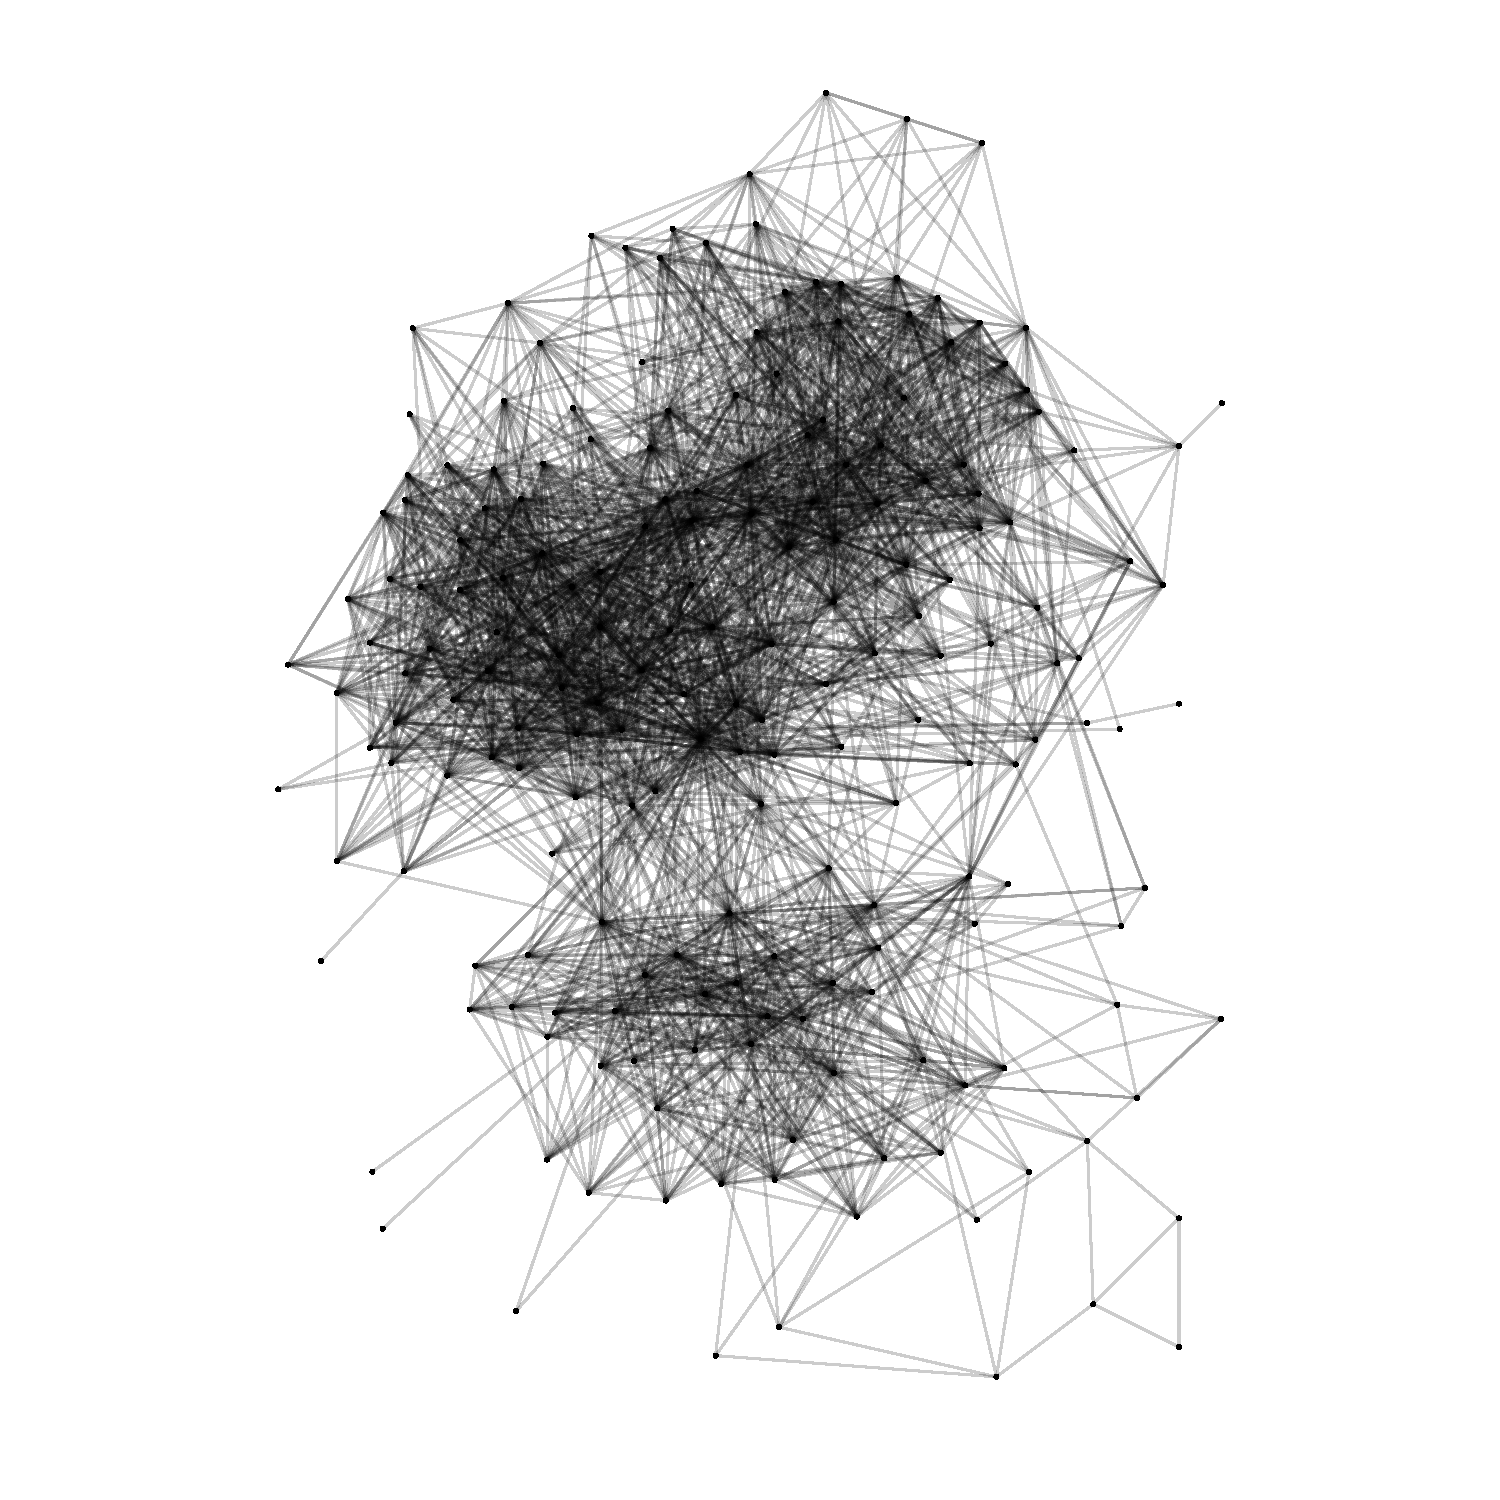
\includegraphics[height=0.7\paperheight]{network-arenas-jazz.pdf}} ;
	\node (university) at (0, 0) {\LARGE \textsc{\univname}} ;
	\node (thesis) at (0, -1.5) {\Large \textsc{\degreename}} ;
	\node[text width=0.6\paperwidth, align=right, anchor=east] (title) at (9, -9) {\Huge\bfseries\ttitle\par} ;
	\node[align=right, anchor=east] (author) at (9, -11) {\textit{Author}\\\authorname} ;
	\node[align=right, anchor=east] (author) at (9, -13) {\textit{Supervisors}\\\supname} ;
	\node (department) at (0, -21.5) {\deptname} ;
	\node (group) at (0, -22) {\groupname} ;
	\node (date) at (0, -23.5) {\today{}} ;
	

\end{tikzpicture}

\end{center}
\end{titlepage}

%--------------------------------------------
%	ABSTRACT PAGE
%--------------------------------------------

\begin{abstract}
\addchaptertocentry{\abstractname} % Add the abstract to the table of contents
\todo[inline]{Write the abstract}
\end{abstract}

%--------------------------------------------
%	LIST OF CONTENTS/FIGURES/TABLES PAGES
%--------------------------------------------

\tableofcontents % Prints the main table of contents

% \listoffigures % Prints the list of figures

% \listoftables % Prints the list of tables

%--------------------------------------------
%   ABBREVIATIONS
%--------------------------------------------

%\begin{abbreviations}{ll} % Include a list of abbreviations (a table of two columns)

%\end{abbreviations}

%--------------------------------------------
%	SYMBOLS
%--------------------------------------------
	
\chapter*{List of Symbols}
\section*{Single layer networks}

\begin{longtable}{m{0.1\textwidth}m{0.55\textwidth}m{0.3\textwidth}}

\textbf{Symbol}	& \textbf{Description} & \textbf{Math. definition} \\
\addlinespace

$c$			& Expectation value for the degree & $\expected{\deg{v}}$ \\
$C$			& A connected component \\
$\deg{v}$	& Degree of vertex $v$ \\
$\deg[1]{v}$	& Degree of a vertex $v$ that has been reached by following an edge \\
$\expected{\dots}$	& Expectation value \\
$g_0(z)$	& Generating function for the degree of uniformly chosen nodes & $\sum_{k=0}^\infty p_k z^k$ \\
$g_1(z)$	& Generating function for the degree of nodes reached by following an edge & $\sum_{k=0}^\infty q_k z^k$ \\
$k_i$	& Degree of vertex $i$ \\
$m$		& Number of edges in the network \\
$n$			& Number of nodes in the network \\
$N(v)$ 		& Neighborhood of a vertex $v$ \\
$p_{ij}$	& Probability that vertices $i$ and $j$ are connected \\
$p_k$		& Probability that a random node has degree $k$ & $P_0(\deg{v} = k)$ \\
$P_0(\dots)$	& Probability starting from a uniformly chosen node \\
$P_1(\dots)$	& Probability starting from a node reached by following an edge \\
$q_k$		& Probability that a node reached by following a edge has degree $k + 1$ & $P_1(\deg{v} = k + 1)$ \\
$r_k$		& Probability that a random node of the GCC has degree $k$ & $P_0(\deg{v} = k | v \in \GCC)$ \\
$S$ 		& Fraction of the network which is part of the GCC in the large $n$ limit & $P_0(v \in \GCC)$ \\
$u$			& Probability that a node reached by following an edge is not part of the GCC & $P_1(v \notin \GCC)$ \\
$v$			& Random variable representing a vertex chosen in a network, either uniformly or by following an edge depending of the context \\

\addlinespace
\addlinespace
\addlinespace

$\alpha$	& Exponent of a power law distribution \\
$\zeta(\alpha)$	& Riemann zeta function \\

\end{longtable}

\newpage

\section*{Multiplex networks}

\emph{For multiplex networks, the convention we follows to indicate a value refer to layer $i$ is to add an upper index $(i)$ if the quantity has a lower index and to add a lower index $i$ otherwise.}

\begin{longtable}{m{0.1\textwidth}m{0.6\textwidth}m{0.25\textwidth}}

\textbf{Symbol}	& \textbf{Description} & \textbf{Math. definition} \\
\addlinespace

$L$ 				& Number of layers of the multiplex network \\
$N$					& Number of parameters determining the degree distributions of a multiplex network \\
$N_i(v)$ 			& Neighborhood of a vertex $v$ in layer $i$ \\
$F(\lambdavec, \zvec)$ & Residual function \\
$F_{\lambdavec}(\zvec)$		& Residual function with fixed parameter vector $\lambdavec$ \\
$g^{(i)}_0(z)$		& Generating function for the degree of uniformly chosen nodes in layer $i$ & $\sum_{k=0}^\infty p^{(i)}_k u_i^k$ \\
$g^{(i)}_1(z)$		& Generating function for the degree of nodes reached by following an edge in layer $i$ & $\sum_{k=0}^\infty q^{(i)}_k u_i^k$ \\
$J_{\lambdavec}(\zvec)$					& Jacobi matrix of $F_{\lambdavec}(\zvec)$ \\
$p^{(i)}_k$			& Probability that a uniformly chosen node has degree $k$ in layer $i$ & $P^{(i)}_0(\deg{v} = k)$ \\
$P^{(i)}_0(\dots)$	& Probability for an event in layer $i$ starting from a uniformly chosen node  \\
$P^{(i)}_1(\dots)$	& Probability for an event in layer $i$ starting from a node reached by following an edge in layer $i$ \\
$q^{(i)}_k$		& Probability that a node reached by following a edge has degree $k + 1$ & $P^{(i)}_1(\deg{v} = k + 1)$ \\
$\mathcal{R}$	& Critical region \\
$u_i$			& Probability that a node reached by following an edge in layer $i$ is not part of the GVC & $P^{(i)}_1(v \notin GVC)$ \\
$\uvec$			& Vector of all $u_i$ & $(u_1, u_2, \dots, u_L)$ \\
$\uvec_T$		& Trivial solution for $\uvec$ & $(1, 1, \dots, 1)$ \\
$\uvec^\dagger$	& Non trivial solution for $\uvec$ \\

\addlinespace
\addlinespace
\addlinespace

$\lambda_j$ 	& One of the $N$ parameters determining the degree distributions of a multiplex network \\
$\lambdavec$	& Parameter vector & $(\lambda_1, \lambda_2, \dots, \lambda_N)$ \\
$\lambdavec^c$	& Parameter vector in the critical region \\
$\psi(\lambdavec, \uvec)$	& Fixpoint function for $\uvec$ \\
$\Psi(\Lambda, U)$			& Interval extension of $\psi(\lambdavec, \uvec)$ \\

\end{longtable}



%--------------------------------------------
%	THESIS CONTENT - CHAPTERS
%--------------------------------------------

\listoftodos

\mainmatter % Begin numeric (1,2,3...) page numbering

\pagestyle{thesis} % Return the page headers back to the "thesis" style


%--------------------------------------------
%	SINGLE LAYER
%--------------------------------------------
\chapter{Single layer networks}
\label{Section: Single layer networks}

\section{Introduction}

Many systems in real world can be conceptually represented as a collection of objects being connected to each other in some way. Such representation is called a \newconcept{network}. For example, a power grid can be represented as stations connected by power lines \cite{watts1998collective}, as shown in fig. \ref{Figure: Network of western US powergrid} for the power grid of western USA. The concept of network does not require the object or the links between them to be physical. As an example, we can represent collaboration as a network: two people are connected if they did collaborate, for example by coauthoring a paper \cite{grossman1995portion}, participate to the same board of direction \cite{davis1997corporate} or having played in the same jazz band \cite{gleiser2003community}. The latter being represented in fig. \ref{Figure: Network of jazz musicians collaborations}. This implies that a very different systems can be represented as networks, from cities connected by road \cite{leskovec2008community, subelj2011robust} (see fig. \ref{Figure: Network euroroad} for an exemple) to proteins connected if they interact \cite{ewing2007large, rual2005towards, stelzl2005human} (see fig. \ref{Figure: Network of human proteins} for a partial network of human proteins), including networks of emails user \cite{guimera2003self, newman2002email}, the internet \cite{albert1999internet} or networks of friendship \cite{foster1963study}. Insight on fundamental properties of networks may therefore shed light on a very broad range of problems. To gain such insights, theoretical studies of general networks, such as the one presented in this thesis, are required.

\begin{figure}
	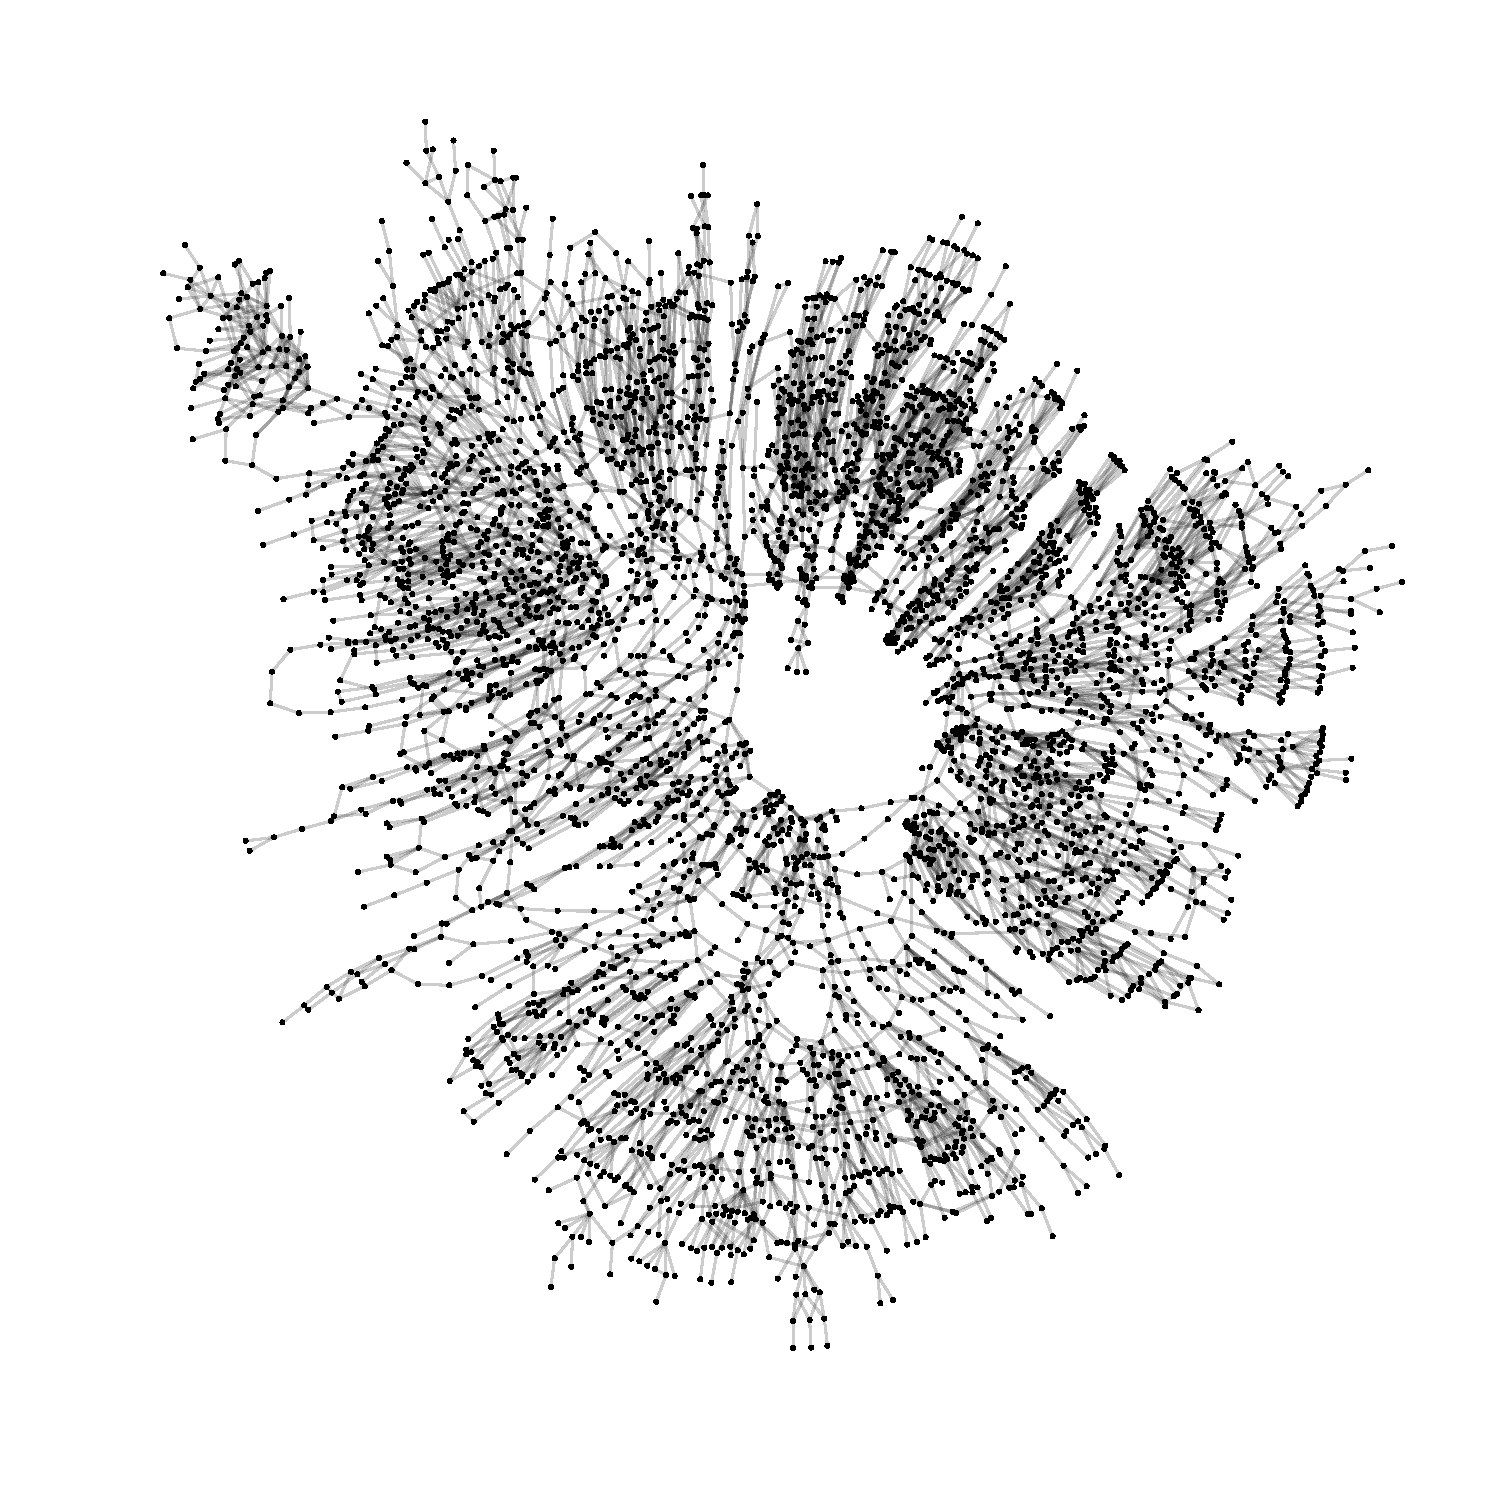
\includegraphics[width=\textwidth]{network-US-power-grid.pdf}
	\caption{Power grid network of the Western States of USA \cite{watts1998collective}. Nodes represent electrical stations (generator, transformator, substation) and edges represent power supply lines. Data retrieved from the Konect database \cite{kunegis2013konect} (Konect code \code{UG}).}
	\label{Figure: Network of western US powergrid}
\end{figure}

\begin{figure}
	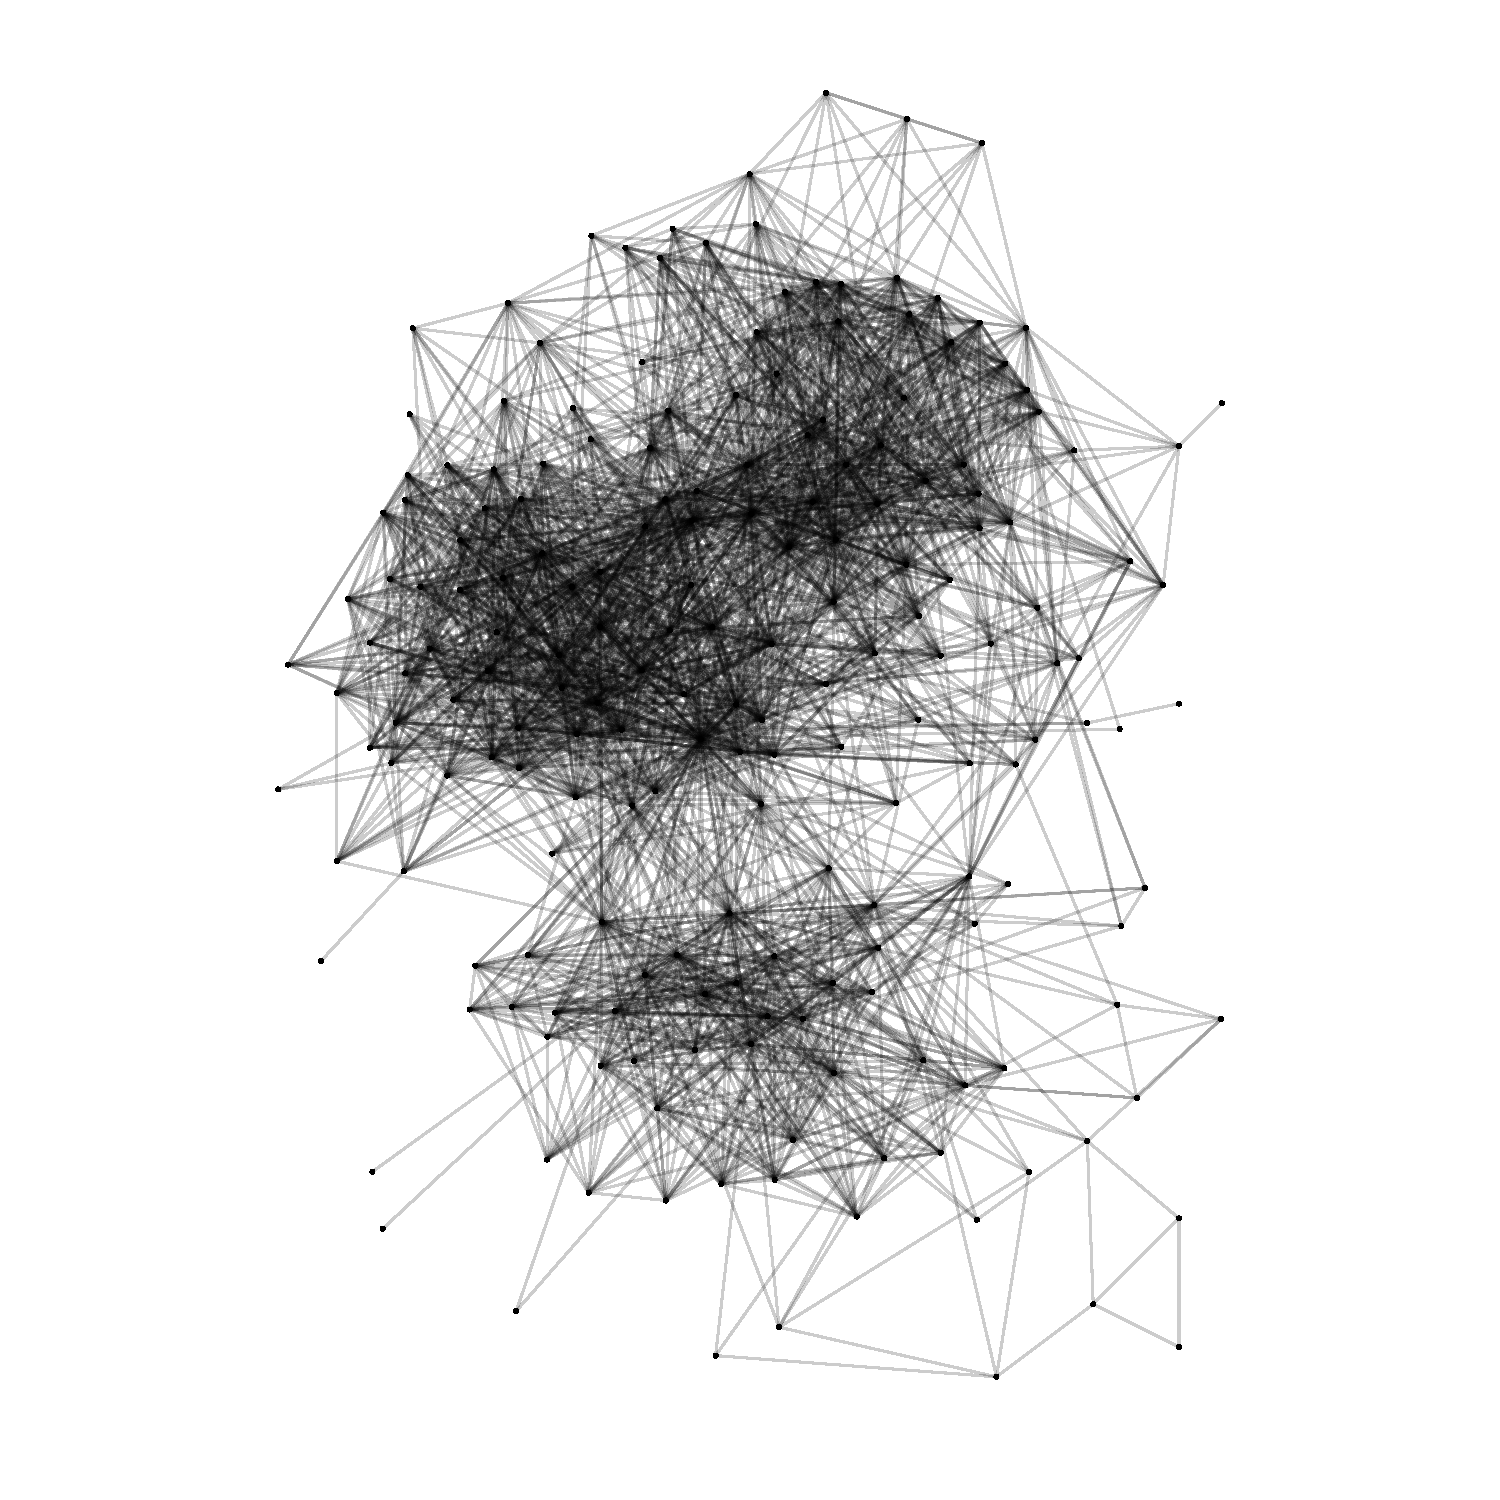
\includegraphics[width=\textwidth]{network-arenas-jazz.pdf}
	\caption{Collaboration network of jazz musicians as of 2003 \cite{gleiser2003community}. Nodes represent musicians and edges represent the fact that the two musicians had played in the same band. Data retrieved from the Konect database \cite{kunegis2013konect} (Konect code \code{JZ}).}
	\label{Figure: Network of jazz musicians collaborations}
\end{figure}

\begin{figure}
	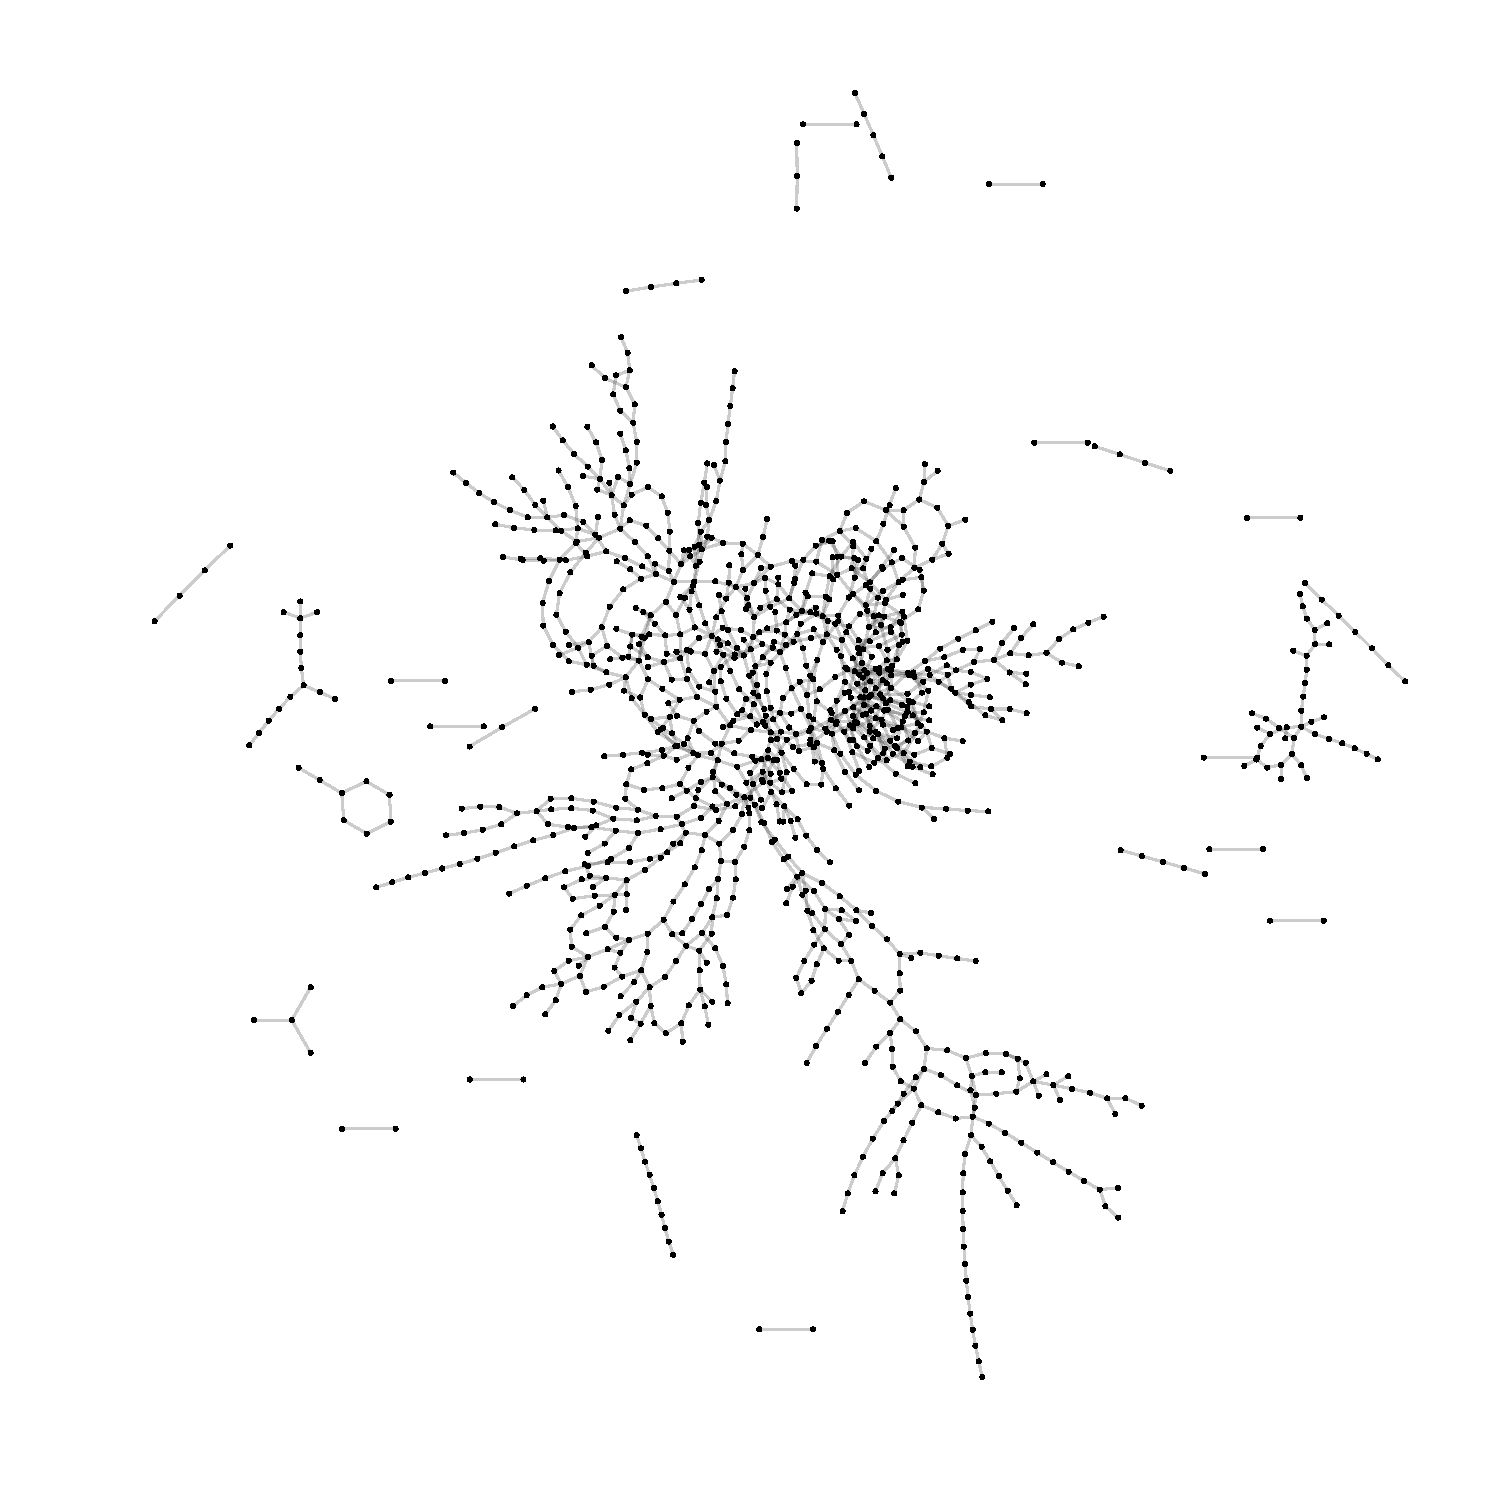
\includegraphics[width=\textwidth]{network-subelj_euroroad.pdf}
	\caption{International E-road network, a network of road situated mainly in Europe \cite{subelj2011robust}. Nodes represent cities and edges represent E-roads connecting them. Data retrieved from the Konect database \cite{kunegis2013konect} (Konect code \code{ET}).}
	\label{Figure: Network euroroad}
\end{figure}

\begin{figure}
	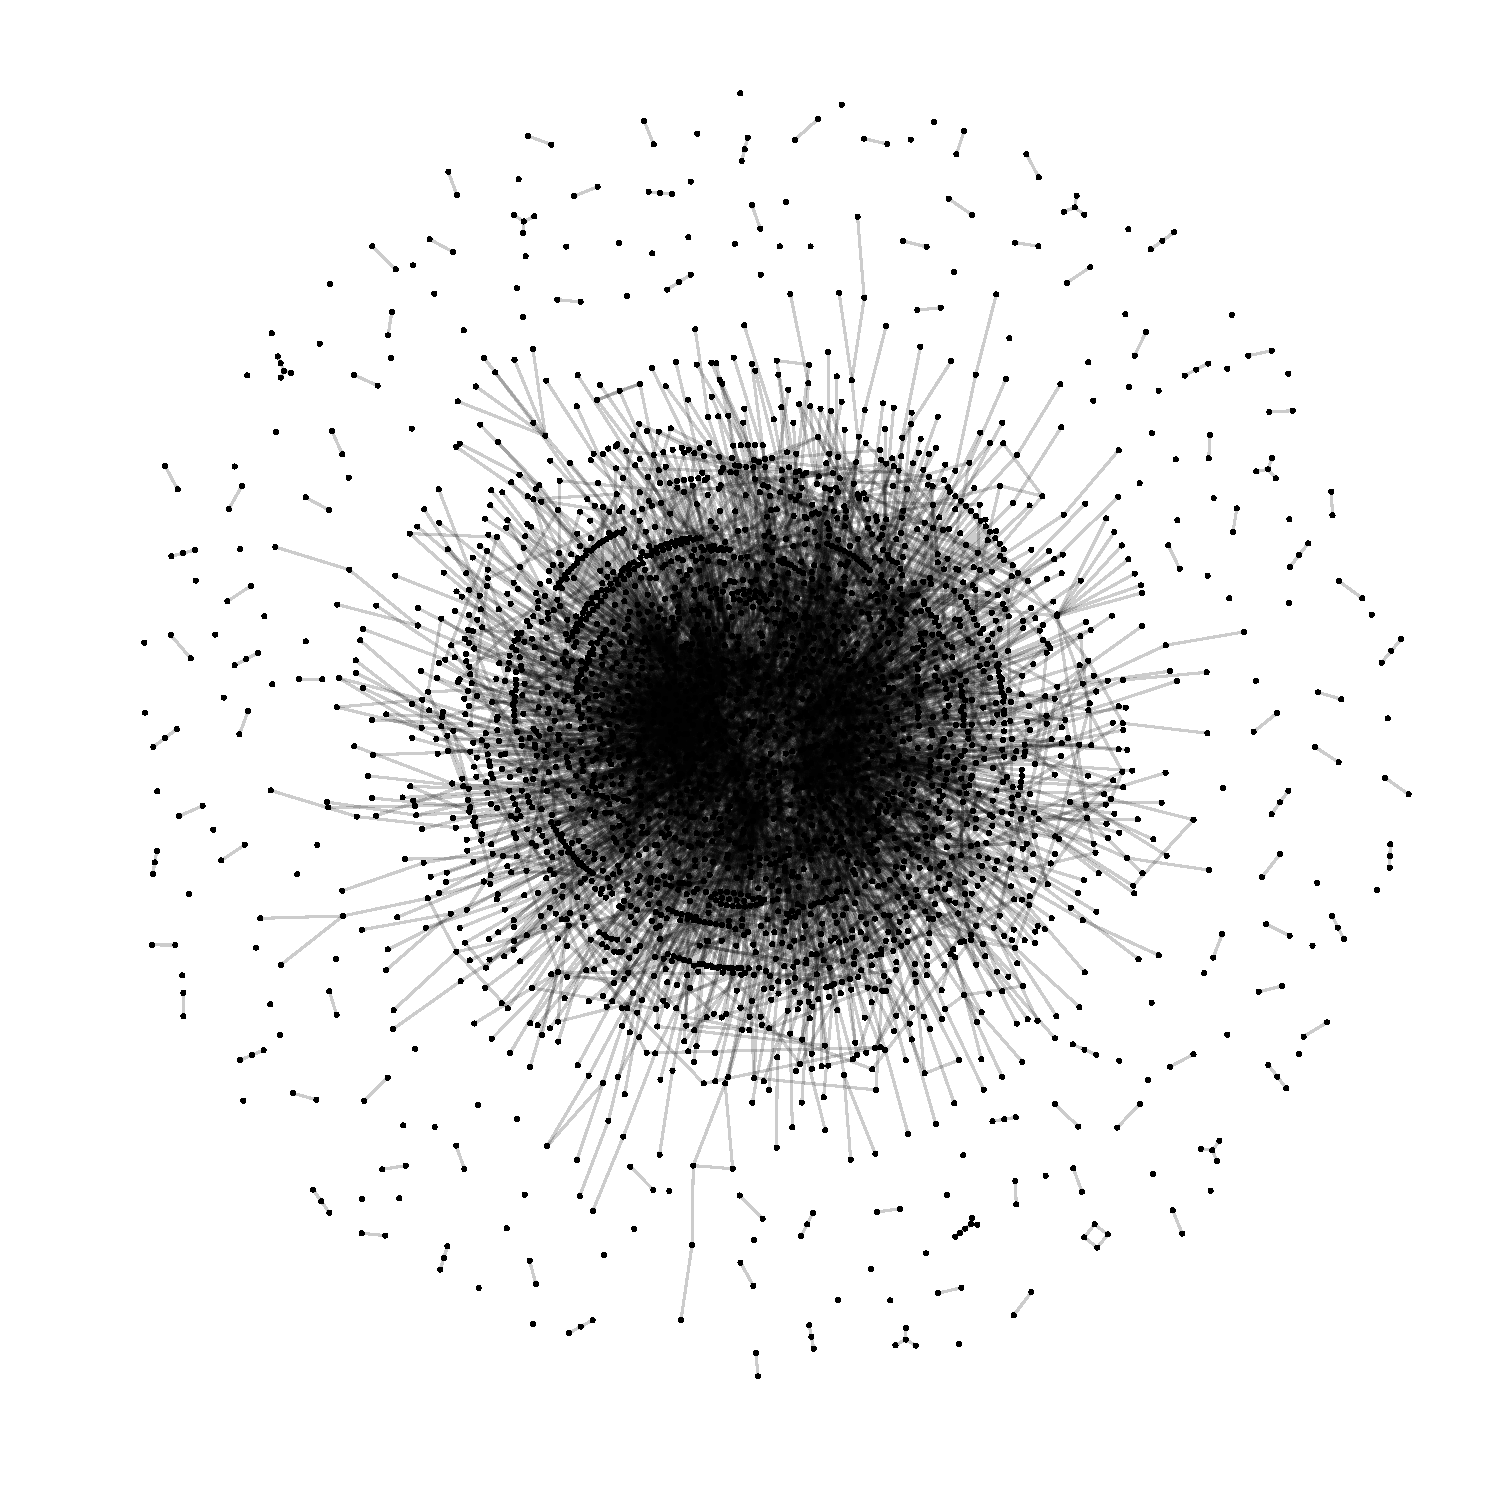
\includegraphics[width=\textwidth]{network-maayan-vidal.pdf}
	\caption{Network of protein-protein interaction in humans \cite{rual2005towards}. Nodes represnt proteins and edges a binary interaction. Data retrieved from the Konect database \cite{kunegis2013konect} (Konect code \code{MV}).}
	\label{Figure: Network of human proteins}
\end{figure}

Mathematically, networks are represented as \newconcept{graphs}. A graph is an object composed of a set $V$ of \newconcept{vertices} (also referred to as nodes) and a set of \newconcept{edges} $E$. An edge is characterized by the fact that it connects two vertices together, which in mathematical terms translates to the fact that an edge can be written as a pair of vertices, or equivalently $E \subset \set{(v_1, v_2) | v_1, v_2 \in V }$. Many extensions of this model exist, for example edges may have a direction (\newconcept{directed graph}), implying that $(v_1, v_2) \neq (v_2, v_1)$, or edges can carry a value (\newconcept{weighted graph}) or multiple types of edges may exist, an extension called multiplex network that is the subject of Chapter \ref{Section: Multiplex networks}.

In this first chapter we mainly follow the presentation given by Newman in Chapter 13 of \cite{newman2010networks} of standard unweighted and undirected networks, except for Sections \ref{Section: Degree distribution in the GCC}, \ref{Section: Exponential networks} and \ref{Section: Generating connected networks} that are addition absent of Newman's book. We further restrict our study to infinitely large networks as it allows for several convenient simplifications while still capturing important feature networks. We first present a general framework for the study of networks, the configuration model, and study several of its properties. Introducing the generating function mathematical tool, we then determine the low and high connectivity phases of networks, and their characteristics. We then apply the presented theory on three types of networks, Erdos-Renyi networks, scale-free networks and networks with exponential degree distribution. Finally, we present and study an algorithm generating fully connected networks.

\section{Configuration model}
\label{Section: Configuration model}

Since we are interested in fundamental properties of networks, we need to abstract from the specificity of single networks. To do so we consider that networks are fully determined by their \newconcept{degree distribution} $\set{p_k}$ where $p_k$ is the probability for a node chosen randomly and uniformly to have degree $k$. Since knowing how a network can be constructed is useful both conceptually and to perform computation on properties of the network, we now present an algorithm called \newconcept{configuration model} \cite{newman2010networks} that sample uniformly the space of all network with a given degree distribution.

Consider a network with $n$ vertices with a given degree distribution $\set{p_k}$. If we cut every edges in two, every vertex keep a number of \newconcept{stubs} (half-edges) equal to its degree. The resulting set of vertices and stubs is independent of the network structure, but common for all networks with the same degree distribution. The idea of this algorithm is thus to start from this state, a set of nodes with stub degree distribution $\set{p_k}$. Then each stub is connected to another chosen uniformly amongst the other stubs to form the edges of the network. By construction, the produced network has degree distribution $\set{p_k}$.

The fact that stubs are paired uniformly and independently is important in that it implies that the vertex reached by following a random edge does not depend, in probability, on the vertex at the starting end of the edge.

A computer algorithm able to simulate configuration model is rather straightforward to implement. First generate $n$ random numbers $k_1, k_2, \dots, k_n$ following the probability distribution $p_k$, one for each node. They are the respective degrees of the nodes. If the total degree $2m = \sum k_i$ is not even, add one node with degree $1$, which has a negligible effect on the degree distribution but allows to have a even number of stubs and thus to connect all of them. Then build a list $\algoset{stubs}$ of the stubs, where each stub is represented by the index of the node to which it is attached. As a consequence, index $i$ is repeated $k_i$ times in $\algoset{stubs}$, and so for each $i$. This stub list is then to be shuffled uniformly\footnote{Most programming languages provide this functionality.}. Finally a node is create for each pairs of indices in $\algoset{stubs}$, i.e. an edges is create between vertex $s_i$ and $s_{i + 1}$ for $i = 1, 3, 5, \dots, 2m - 1$. This procedure ensures that the stubs are paired uniformly and thus that it is equivalent to the configuration model.

Finally since $\set{p_k}$ is a probability distribution, it is independent of the number of nodes $n$ of the network, we can consider the limit for large $n$. In this thesis we only consider this limit as it allows several mathematical simplifications while still capturing the essential structure of a network. Moreover for sufficiently large networks, the difference between the large $n$ limit and the actual network is small and can thus safely be neglected.

\begin{figure}
	{
\newcommand{\configurationmodelexamplepoints}
{
	\node[node] (A) at (0.2, 0) {} ;
	\node[node] (B) at (1, 1.5) {} ;
	\node[node] (C) at (-0.7, 1.2) {} ;
	\node[node] (D) at (-0.5, -0,1) {} ;
	\node[node] (E) at (1.7, -0.6) {} ;
}

\newcommand{\legendpos}{(0.2, -1.5)}


\begin{tikzpicture}
	\configurationmodelexamplepoints
	
	\draw (A) -- ++(0.4, 0.3) ;
	\draw (A) -- ++(-0.5, 0) ;
	\draw (A) -- ++(-0.3, 0.4) ;
	
	\draw (B) -- ++(0.4, -0.3) ;
	\draw (B) -- ++(-0.4, -0.3) ;
	
	\draw (C) -- ++(-0.3, -0.4) ;
	\draw (C) -- ++(0.5, 0) ;
	
	\draw (D) -- ++(-0.3, 0.4) ;
	
	\draw (E) -- ++(-0.4, -0.3) ;
	\draw (E) -- ++(0, 0.5) ;
	
	\node (leg) at \legendpos {(A) Nodes and theirs stubs} ;
\end{tikzpicture}
\hspace{1cm}
\begin{tikzpicture}
	\configurationmodelexamplepoints
	
	\draw (A) -- (B) ;
	\draw (A) -- (C) ;
	\draw (A) -- (E) ;
	\draw (B) -- (E) ;
	\draw (C) -- (D) ;
	
	\node (leg) at \legendpos {(B) Stubs are randomly connected} ;
\end{tikzpicture}
}
	\caption{Schematic representation of the configuration model.}
	\label{Figure: Configuration model}
\end{figure}

\section{Self-edges and multi-edges}

Using the insight given by the algorithm, we can compute the probability that a node is connected to itself, thus making a so-called \newconcept{self-edge}. First note that in the limit of large $n$, the number of vertices with degree $k$ is equal to $n p_k$ and as a consequence the total number $m$ of edges is equal to
\begin{align}
	m = \frac{1}{2} \sum_{k = 0}^\infty n k p_k = \frac{n}{2} \expected{\deg{v}}, \label{Total number of edges}
\end{align}
with $\expected{\dots}$ denoting the expectation value

The probability that an edge connect node $i$ with degree $k_i$ to itself is equal to the number of way to connect both ends of the edge to this node $k_i (k_i - 1)$, divided by the number of way an edge can be placed in the network $2 m (2 m - 1)$. Multiplying this by the number of edges $m$ gives the probability $p_{ii}$ that node $i$ is connected to itself
\begin{align}
	p_{ii} = \frac{k_i (k_i - 1)}{2 (2m - 1)},
\end{align}
The total number of self-edges is
\begin{align}
	\sum_{i=1}^n p_{ii} &= \sum_{i=1}^n \frac{k_i^2 - k_i}{2 (2m - 1)} \\
		&= \frac{1}{2} \frac{\expected{(\deg{v})^2} - \expected{\deg{v}}}{n \expected{\deg{v}} - 1}.
\end{align}
Since we are considering a constant degree distribution $p_k$ all expectations value remain constant when $n$ grows, so the number of vertices having self edges goes to zeros as $n$ becomes large and we can safely consider that the generated network has no self-edges at all.

Similarly, we find that the probability $p_{ij}$ that two vertices $i$ and $j$ are connected is equal to
\begin{align}
	p_{ij} = m \frac{k_i k_j}{ \begin{pmatrix} 2m - 2 \\ 2 \end{pmatrix} } = \frac{k_i k_j}{2 m -1}.
\end{align}
The probability to have two or more edges between the vertices $i$ and $j$ is equal to the probability that $i$ and $j$ are connected and that they remain so after we remove one edge between them. The probability for them to be connected with one edge less is the same as $p_{ij}$ but with one edge less in total and one stub less at both $i$ and $j$, giving
\begin{align}
	\frac{(k_i - 1)(k_j - 1)}{2 m - 3}.
\end{align}
In consequence we find the probability to have at least two edges between $i$ and $j$ to be
\begin{align}
	p_{ij} \frac{(k_i - 1)(k_j - 1)}{2 m - 3} = \frac{k_i k_j (k_j - 1) (k_i - 1)}{2 (2 m - 1)(2 m - 3)}.
\end{align}
Summing over all vertex pairs and dividing by two to avoid double counting the pairs, we find that the total expected number of multi-edges is
\begin{align}
	\frac{\sum_{ij} k_i k_j (k_j - 1) (k_i - 1)}{2 (2 m - 1)(2 m - 3)}  &\approx \frac{1}{8 m^2} \sum_i k_i(k_i - 1) \sum_j k_j(k_j - 1) \\
	&= \frac{1}{2}\left[ \frac{\expected{(\deg{v})^2} - \expected{\deg{v}}}{\expected{\deg{v}}} \right]^2,.
\end{align}
The approximation holds since in the limit of large $n$ we have $2 m - 3 \approx 2 m - 3 \approx 2 m$ as $m$ scale proportionally to $n$. The number of multi-edges is thus asymptotically constant and we can therefore consider that the generated networks has no multi-edges, since the fraction of affected nodes goes to zero in the limit of large $n$.

A network having this two properties, absence of self-edges and of multi-edges, is said to be a \newconcept{simple graph}. Since for $n$ large enough all networks in the context of the configuration model have approximately these two properties, we always consider that the networks are simple graphs in the remaining of this thesis.

\section{Uniformity of network space sampling}

In the previous section we demonstrated that the configuration model asymptotically produces simple graphs in the limit of large $n$. This is necessary to prove the claims we make in Section \ref{Section: Configuration model} that the configuration uniformly sample the space of networks with a given degree distribution. To prove that claim is equivalent to prove that each different simple network appears with the same probability.

A \emph{matching} of the stubs is a possible way to connect $2 m$ distinguishable stubs. By construction the pair of stubs that are bound are chosen uniformly and thus each matching appears with the same probability than any other. However, in practice the stubs of a single vertex are not distinguishable, nor are the vertices of the same degree, so several matching leads to the same network. There are $k!$ way of arranging the stubs of a vertex of degree $k$, and $(n p_k)!$ way of arranging the $n p_k$ nodes of degree $k$ (in the limit of large $n$) resulting in a total of
\begin{align}
	\prod_{i = 1}^n k_i! \prod_{k = 0}^\infty (n p_k)!
\end{align}
matchings corresponding to the same network, where $k_i$ is the degree of vertex $i$\footnote{This value differs from the one given by Newman in \cite{newman2010networks} as he does not take in account the indiscernibility of vertices with the same degree, but this does not change the conclusion.}. This quantity only depends on the degree distribution, thus all networks with the same degree distribution have the same number of different matchings. Since each matching appears with the same probability, we can conclude that each network with a given degree distribution appears with the same probability in the configuration model.

In a sense the configuration model is therefore optimal for the point of view we adopt in this thesis. Indeed we consider a network fully determined by its degree distribution and all network with a common degree distribution are equal with regard to the configuration model as it sample them uniformly. We could in fact present the configuration model as a consequence of the requirement that we want a sampling method introducing no unnecessary constrain on the produced networks. See Section 15.2 of \cite{newman2010networks} or Section 2 of \cite{bauer2002maximal} for discussions of that point of view.

\section{Excess degree distribution}

As we will see below, while we consider that a network is fully determined by its degree distribution, considering vertices reached by following an edge gives valuable insights on the network structure. We call such vertex a \newconcept{first neighbor} vertex and we denote $P_1(\dots)$ the probability associated with a first neighbor, while we denote $P_0(\dots)$ the probability associated with uniformly chosen vertices\footnote{In principle $P_j(\dots)$ could be defined, corresponding to the probability associated with vertices reached after following $j$ edges.}. We can define the \newconcept{excess degree distribution} $\set{q_k}$ as
\begin{align}
	q_k = P_1(\deg{v} = k + 1), \qquad \forall k \in \mathbb{N}.
\end{align}
The probability $q_k$ correspond to a first neighbor having degree $k + 1$, or equivalently to the probability to have $k$ edges other than the on used to reach the node in the first place, hence the name excess degree distribution.

The excess degree distribution can be computed explicitly by noting that a stub has the same probability to be connected to any if the other $2 m - 1$ stubs, thus the probability that this stub is connected to a given node of degree $k$ is $k/(2 m - 1)$. Multiplying by the total number of node of degree $k$, $n p_k$ in the large $n$ limit,gives the probability that a given node is attached to a node of degree $k$ as
\begin{align}
	\frac{k}{2 m -1} n p_k = \frac{k p_k}{\expected{\deg{v}}}.
\end{align}
Since $q_k$ is the probability that a first neighbor has degree $k + 1$, we can conclude
\begin{align}
	q_k = \frac{(k + 1) p_{k+1}}{\expected{\deg{v}}}. \label{qk as function of pk}
\end{align}

\section{Generating functions}
\label{Section: Generating functions}

A powerful way of representing a discrete probability law (or any sequence of number) is the \newconcept{generating function} of the distribution \cite{wilf2005generatingfunctionology}. For a degree distribution $\set{p_k}$ it is defined as the function
\begin{align}
	g_0(z) = \sum_{k=0}^\infty p_k z^k. \label{Definition of g0}
\end{align}
The fact that $p_k$ is a probability distribution implies that
\begin{align}
	\sum_{k = 0}^\infty p_k = 1, \label{Normalization of pk}
\end{align}
hence the infinite sum in eq. \eqref{Definition of g0} always converges for $\rvert z \rvert \leq 1$, which allows to numerically evaluate $g_0(z)$ in that range.

Observe that the derivative with respect to $z$ of $g_0(z)$ is
\begin{align}
	g'_0(z) = \sum_{k=0}^\infty p_k k z^{k-1}. \label{Derivative of g0}
\end{align}
Comparing with the definition of the expectation value we find
\begin{align}
	\expected{\deg{v}} = \sum_{k=0}^\infty p_k k = g'_0(1). \label{Expectation value as g'0(1)}
\end{align}
Therefore, the generating function is sufficient to know the expectation value of a distribution. This result can be generalized: if we look at the second derivative of the generating function, by differentiating eq. \eqref{Derivative of g0}, we find
\begin{align}
	g''_0(1) &= \sum_{k=0}^\infty p_k k (k - 1) = \sum_{k=0}^\infty p_k k^2 - \sum_{k=0}^\infty p_k k \\
		&= \expected{(\deg{v})^2} - \expected{\deg{v}}. \label{Second derivative of g0}
\end{align}
Thus we can write
\begin{align}
	\expected{(\deg{v})^2} &= g''_0(1) + g'_0(1) = \frac{\partial}{\partial z}\left(z g'_0(z)\right)\evaluatedat{z = 1},  \label{Second moment as derivatives of g0}
\end{align}
which means that the second moment is fully determined by the generating as well. In fact such formula exists for all moments, but we do not present it here as in this thesis we use at most the first two moments.

All these properties do not depend on the degree distribution $p_k$ to which the generating function is associated and apply to any discrete probability distribution. One other important distribution for network is the excess degree distribution $\set{q_k}$, we define its generating function $g_1$ as
\begin{align}
	g_1(z) = \sum_{k=0}^\infty q_k z^k. \label{Definition of g1}
\end{align}

Inserting eq. \eqref{qk as function of pk} in this definition, we get
\begin{align}
	g_1(z) = \frac{1}{\expected{\deg{v}}} \sum_{k=0}^\infty (k + 1) p_{k + 1} z^k = \frac{g'_0(z)}{g'_0(1)}, \label{g1 as a function of g0}
\end{align}
where we used eq. \eqref{Expectation value as g'0(1)} and eq. \eqref{Derivative of g0 for scale free networks}  to obtain the last equality.

Similar to eq. \eqref{Expectation value as g'0(1)} we find the expected value of the excess degree distribution as
\begin{align}
	g'_1(1) = \frac{g''_0(1)}{g'_0(1)} = \frac{\expected{(\deg{v})^2}}{\expected{\deg{v}}} - 1,
\end{align}
where we inserted the expression in eq. \eqref{Second derivative of g0} for the second derivative of $g_0(z)$. Recall that the excess degree distribution count one edge less than the degree of a vertex $v$, we can find the mean degree of first neighbors as
\begin{align}
	\expected{\deg[1]{v}} = g'_1(1) + 1 = \frac{\expected{(\deg{v})^2}}{\expected{\deg{v}}}, \label{Average degree of neighbor as second moment}
\end{align}
where we use $\deg[1]{v}$ to denotes the degree of a first neighbor. By introducing the variance of the degree distribution
\begin{align}
	\var{\deg{v}} &= \expected{(\deg{v})^2} - \left(\expected{\deg{v}}\right)^2 \\
\end{align}
and replacing the second moment in eq. \eqref{Average degree of neighbor as second moment} we find a new expression for the average degree of first neighbors
\begin{align}
	\expected{\deg[1]{v}} = \expected{\deg{v}} + \frac{\var{\deg{v}}}{\expected{\deg{v}}}.
\end{align}
Using this form, it is manifest that the average degree and the average degree of first neighbor differ. Precisely they difference depend on the variance of the degree distribution, which has one immediate striking consequence: since both the average degree and its variance are non negative, we have in general
\begin{align}
	\expected{\deg[1]{v}} \geq \expected{\deg{v}}. \label{Friends of friends inequality}
\end{align}
In other words, as Feld put it in the name of his original paper on the subject, this explains "why your friends have more friends than you do" \cite{feld1991friends}. Note that this feature is universal. We present it here in the context of the configuration model, but inserting the degree distribution of any network in the calculations presented leads to same result.

\section{Giant connected component}
\label{Section: Giant connected component}

\subsection{Size of the GCC}

An interesting property of a network is the presence and size of \newconcept{connected components}. A set of nodes is said to be connected if there is a path formed of successive edges from any of its node to any other. All networks can be divided in connected components such that all nodes are element of exactly one component, as it is exemplified in fig. \ref{Figure: Connected components}. The connectedness of network is crucial in many real world realisations of networks. In particular any logistic network, such as power grid networks, rail road network or the internet network, is functional only if it is able to transfer goods or services (electricity, passengers or informations) from any node to any other.

\begin{figure}
	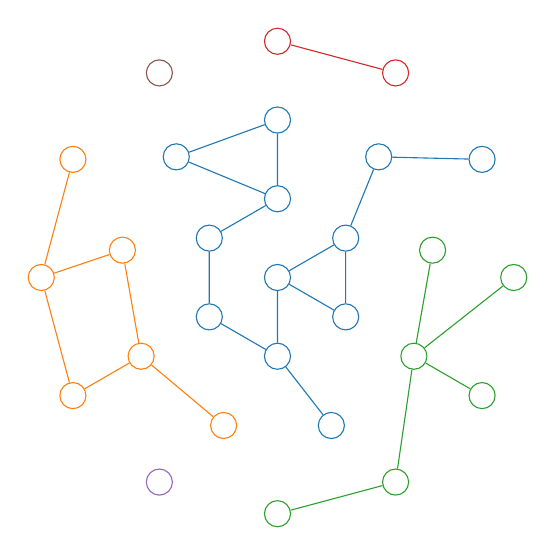
\begin{tikzpicture}
	\node (A') at (0, 0) {} ;
	
	\foreach \n in {1, 2, ..., 6}
	{
		\node (B\n') at ({sin(\n*360/6)}, {cos(\n*360/6)}) {} ;
	}
	
	
	\foreach \n in {1, 2, ..., 9}
	{
		\node (C\n') at ({2*sin(\n*360/9)}, {2*cos(\n*360/9)}) {} ;
	}
	
	
	\foreach \n in {1, 2, ..., 12}
	{
		\node (D\n') at ({3*sin(\n*360/12)}, {3*cos(\n*360/12)}) {} ;
	}
	
	\newcommand{\compcolor}{C0}
	\foreach \cooname in {A, B1, B2, B3, B4, B5, B6, C1, C4, C8, C9, D2}
	{
		\node[node, \compcolor] (\cooname) at (\cooname') {} ;
	}
	\draw[\compcolor] (A) -- (B1) -- (B2) -- (A) ;
	\draw[\compcolor] (A) -- (B3) -- (C4) ;
	\draw[\compcolor] (B1) -- (C1) -- (D2) ;
	\draw[\compcolor] (B3) -- (B4) -- (B5) -- (B6) -- (C9) -- (C8) -- (B6) ;
	
	
	\renewcommand{\compcolor}{C1}
	\foreach \cooname in {C5, C6, C7, D8, D9, D10}
	{
		\node[node, \compcolor] (\cooname) at (\cooname') {} ;
	}
	\draw[\compcolor] (D10) -- (D9) -- (D8) -- (C6) -- (C7) -- (D9) ;
	\draw[\compcolor] (C6) -- (C5) ;
	
	
	\renewcommand{\compcolor}{C2}
	\foreach \cooname in {C2, C3, D3, D4, D5, D6}
	{
		\node[node, \compcolor] (\cooname) at (\cooname') {} ;
	}
	\draw[\compcolor] (C2) -- (C3) -- (D5) -- (D6) ;
	\draw[\compcolor] (D3) -- (C3) -- (D4) ;
	
	
	\renewcommand{\compcolor}{C3}
	\foreach \cooname in {D1, D12}
	{
		\node[node, \compcolor] (\cooname) at (\cooname') {} ;
	}
	\draw[\compcolor] (D12) -- (D1) ;
	
	
	\node[node, C4] (D7) at (D7') {} ;
	\node[node, C5] (D11) at (D11') {} ;
\end{tikzpicture}
	\caption{Scheme of a graph with six connected components, each drawn with a different color.}
	\label{Figure: Connected components}
\end{figure}

Insight on the property of networks can be found by studying the case where the fraction of the network occupied by a connected component does not vanish in the large $n$ limit. Such component is called a \newconcept{giant connected component} (GCC).

To get informations about the GCC we first compute the fraction occupied by an arbitrary connected component $C$ of the network. We can write the probability $S$ that a randomly chosen vertex is part of $C$ as
\begin{align}
	S 	&= 1 - P_0(w \notin C\; \forall w \in N(v))\\
		&= 1 - \sum_{k=0}^\infty P_0(w \notin C\; \forall w \in N(v)|\deg{v} = k) P_0(\deg{v} = k).
\end{align}

The probability $P_0(w \notin C\; \forall w \in N(v)|\deg{v} = k)$ is the probability that no neighbors of a node with degree $k$ are part of the component $C$. This in turn is the probability that by following the $k$ edges going out of vertex $w$ we we find each time a node which is not part of $C$. However, as mentioned at the end of Section \ref{Section: Configuration model}, by construction of the configuration model, the vertex at the end of an edge does not depend on the vertex at the other end. Therefore, we can consider the $k$ edges attached to $w$ to be independent, which allow us to write
\begin{align}
	P_0(w \notin C\; \forall w \in N(v)|\deg{v} = k) = \left[P_1(w \notin C)\right]^k = u^k. \label{Probability that a node of degree k is not in the GCC}
\end{align}
In the last equality we introduce the probability $u$ that a node reached by following an edge is not part of $C$,
\begin{align}
	u = P_1(w \notin C). \label{Definition of u}
\end{align}

Noting that $P_0(\deg{v} = k) = p_k$, we finally find
\begin{align}
	S	&= 1 - \sum_{k=0}^\infty u^k p_k \\
		&= 1 - g_0(u).
\end{align}

We now have a compact expression for $S$ in terms of $u$ and the generating function of the degree distribution $g_0$. To determine $u$ we observe that if a vertex $v$ is not part of $C$, none of its neighbors is either. By definition of $u$ this was already known for the node at the other end of the edge from where $v$ was reached. Thus there are only $\deg{v} - 1$ to take in account when computing the probability $v$ is not part of $C$. Using this observation we can express $u$ as
\begin{align}
	u 	&= P_1(w \notin C \; \forall w \in N(v)) \\
		&= \sum_{k=1}^\infty P_1(w \notin C \; \forall w \in N(v)| \deg{v} = k - 1) P_1(\deg{v} = k - 1) \\
		&= \sum_{k=0}^\infty u^k q_k \\
		&= g_1(u),
\end{align}
where we use eq. \eqref{Probability that a node of degree k is not in the GCC} again together with the fact that by definition of the excess degree distribution $q_k = P_1(\deg{v} = k + 1)$.

We end up with two equations to describe the size of a connected component
\begin{align}
	S = 1 - g_0(u) \label{Single layer S final} \\
	u = g_1(u). \label{Single layer u final}
\end{align}
If we can solve the second one we immediately get the size of the connected component $C$. These results were first derivated in an alternative form by Molloy and Reed in \cite{molloy1995critical} and then presented in the framework of generating functions and extended by Newman \etal{} in \cite{newman2001random}\footnote{The results and derivations that first appeared in \cite{newman2001random} are fully reproduced, with additions and clarifications, by Newman in Chapter 13 of \cite{newman2010networks}. As such we prefer to cite the latter when no historical motivation dictate otherwise.}

However eq. \eqref{Single layer u final} only gives $u$ implicitly and its form strongly depends on the degree distribution, therefore no general analytical solutions can be given. From its graphical representation, shown in fig. \ref{Figure: Solution of of u = g1(u) graphically}, we can see that it has at most two solutions. First the trivial solution $u = 1$ is always present, as by the definition \eqref{Definition of g1} of $g_1(z)$, we have $g_1(1) = 1$, implying $S = 0$. The components described by this regime are not giant connected components, as their relative size $S$ vanish in the large $n$ limit. We do not discuss it further here, but the full component size distribution can be analyzed \cite{newman2010networks, kryven2017general}.

Then in some cases, another solution exists with $u < 1$ and $S > 0$. This solution correspond to the GCC. Moreover, if a GCC exists it is unique. To see that consider a network with two GCC with degree distribution such that $p_k \neq 0$ for some $k \geq 2$\footnote{If $p_k = 0$ for all $k \geq 2$, all nodes have degree $0$ or $1$ and thus the biggest component is at most of absolute size $2$, making clear that no GCC can exist.}. The probability $P_c$ that a node $v$ of degree $k$ connects both GCC is strictly smaller than one. Indeed if $P_c$ was one, it would imply that all nodes are part of the GCC and thus that the GCC is unique.

Finally, in the limit of large $n$, the number of vertices of degree $k$ is $n p_k$ and hence the probability that no degree $k$ vertex connect both GCC is
\begin{align}
	(1 - P_c)^{n p_k}.
\end{align}
Since we assumed $p_k > 0$ and since $P_c < 1$, this probability goes to zero in the limit of large $n$. Therefore we can conclude that the GCC, if it exists, is unique.

The appearance of the GCC, can be seen as a phase transition from a low connectivity phase to a highly connected one. In this context it is natural to search the critical point $\mathcal{R}$ of this transition. To find it observe that, as can be seen on fig. \ref{Figure: Solution of of u = g1(u) graphically}, the $g_1(z)$ curve must "go below" the identity curve at $z = 1$ to create a non trivial solution. This requirement means that the slope of $g_1(z)$ at $z = 1$ must be greater than the slope of the identity, which is $1$. In term of the derivative of $g_1(z)$ the condition is thus $g'_1(1) > 1$ to have a non trivial solution to eq. \eqref{Single layer u final}. Therefore the critical parameter $\mathcal{R}$ for which a GCC appears is defined by the boundary condition
\begin{align}
	g'_1(1) = 1. \label{Boundary condition for single layer}
\end{align}

We can rewrite this condition in term of statistical properties of the network by using eq. \eqref{g1 as a function of g0}, which yields
\begin{align}
	g'_1(1) &= \left[ \frac{\partial}{\partial z} \frac{g'_0(z)}{g'_0(1)} \right]_{z = 1} \\
		&= \frac{g''_0(1)}{g'_0(1)} \\
		&= \frac{1}{\expected{\deg{v}}} \left( \expected{(\deg{v})^2} - \expected{\deg{v}} \right)
\end{align}
For the last equality we used the relation between the first and second moment of the degree distribution and the generating function, $g_0(z)$ given in eq. \eqref{Expectation value as g'0(1)} and \eqref{Second derivative of g0}. Inserting in eq. \eqref{Boundary condition for single layer} and rearranging we find
\begin{align}
	\expected{(\deg{v})^2} - 2 \expected{\deg{v}} = 0.
\end{align}
This condition for the critical point of the phase transition between the low and high connectivity phases was first proved in the general case by Molloy and Reed in \cite{molloy1995critical}. In this paper, they also proved that in the high connectivity phase, where non trivial solution to eq. \eqref{Single layer u final} exist, a GCC must actually be present and that it must be unique. For a proof of this using the generating function formalism see Section 13.6 of \cite{newman2010networks}.

Finally eq. \eqref{Single layer u final} can be solved numerically by noticing that the solution $u$ is a fixpoint of the function $g_1(z)$. Since all coefficients in eq. \eqref{Definition of g1} are non negative, $g_1(z)$ and all its derivative are positive for $z > 0$. As a consequence starting from $z_0 = 0$, the sequence $z_k$ defined by the iteration
\begin{align}
	z_{k + 1}  = g_1(z_k)  \label{Single layer fixpoint g1 iteration}
\end{align}
always converges toward the smallest solution of eq. \eqref{Single layer u final}.

\begin{figure}
	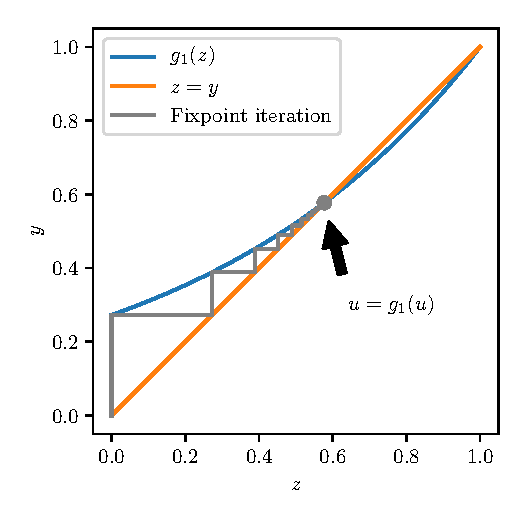
\includegraphics[scale=1]{u_solution_graphically.pdf}
	\caption{Graphical representation of eq. \eqref{Single layer u final} for an Erdos-Renyi network with $c = 1.3$. Gray solid line represent the successive steps of the fixpoint iteration.}
	\label{Figure: Solution of of u = g1(u) graphically}
\end{figure}

\subsection{Algorithm to find the connected components}
\label{Section: Algorithm to find the GCC}

Since we are working in the limit of large $n$, the networks we are generating and analysing have large $n$ as well. Therefore the algorithm we use must be designed with some care to avoid consuming to much computing time, which would make them impractical to use. This motivate us to present the algorithm we use here.

To find all connected components of a network we proceed as follow
\begin{enumerate}
	\item Add all nodes to the set $\mathcal{S}\longsub{unprocessed}$ of unprocessed nodes.
	\item Remove one node from $\mathcal{S}\longsub{unprocessed}$ and add it to the set $\mathcal{S}\longsub{queued}$ of queued nodes.
	\item Start a new component $C$.
	\item Remove one node from $\mathcal{S}\longsub{queued}$ nodes and name it $v$.
	\item Add $v$ to the current component $C$.
	\item Add all unprocessed neighbors of $v$ to $\mathcal{S}\longsub{queued}$.
	\item If $\mathcal{S}\longsub{queued}$ is not empty go to 4, else store the component $C$ and continue.
	\item If $\mathcal{S}\longsub{unprocessed}$ is not empty go to 2, else terminate.
\end{enumerate}
This algorithm goes through each node exactly once and is thus of complexity $\bigO{n}$ which is the optimal complexity since all nodes must be associated to a component.

However, to ensure that the algorithm is fast we must be to efficiently find all neighbors of a node. To do that we represent the network as an \newconcept{adjacency list}: each node is given an index $i$ and the adjacency list $A_i$ contains all the neighbors of $i$. The whole network is thus represented as a list of adjacency list $A = (A_1, \dots, A_n)$.\footnote{For better performance during the creation of the network, our implementation goes a step further and actually request sorted adjacency lists.}

Other representation of networks exist, which are more convenient and efficient for some purposes. However we do not use them in this thesis and we stick to the adjacency list representation.

\subsection{Degree distribution in the GCC}
\label{Section: Degree distribution in the GCC}

Per Bayes theorem we have for two random events $A$ and $B$
\begin{align}
	P(A | B) = P(B | A) \frac{P(A)}{P(B)}. \label{Bayes theorem}
\end{align}
We can apply it to compute the probability $r_k$ that a vertex in the GCC has degree $k$
\begin{align}
	r_k &= P\left(\deg{v} = k | v \in GCC\right)\\
	&= P(v \in GCC | \deg{v} = k) \frac{P(\deg{v} = k)}{P(v \in GCC)} \\
	&= \frac{p_k}{S} \left(1 - P(v \notin GCC | \deg{v} = k)\right) =  \frac{p_k}{S} (1 - u^k). \label{Degree distribution in GCC}
\end{align}
To get the final result we used eq. \eqref{Probability that a node of degree k is not in the GCC}. This result was previously presented more generally and following a very different path by Bauer and Bernard in \cite{bauer2002maximal}.

Therefore we see that considering a vertex in the GCC biases the probability that it has degree $k$ by a factor $(1 - u^k)/S$ as compared to choosing a vertex uniformly in the network. Since both $u$ and $S$ are smaller than $1$, the net effect is to lower the proportion of low degree vertices in the GCC and thus to increase the proportion of high degree vertices. This result can be understood intuitively since in the configuration model the stubs are connected independently. Therefore each edge of a node increases the probability that this node is connected to the GCC, making high degree node over represented in the GCC.

\section{Erdos-Renyi networks}

Erdos-Renyi networks refer to networks build using the first model of random graphs studied in the literature. This model was probably first introduced in 1951 by Solomonoff and Rapoport \cite{solomonoff1951connectivity} and latter popularized (and probably independantly rediscovered) by Gilbert \cite{gilbert1959random} and Erdos and Renyi \cite{erdos1959random}, the latter giving it their name as they further studied it in the subsequent years \cite{erdos1960evolution, erdos1961strength}. The model grows a network as follow: for each pair of nodes $i$ and $j$, an edge is added with fixed probability $p$.

To find the degree distribution in such network, first notice that the expected degree, usually denoted $c$ for Erdos-Renyi network, is equal to the number of other vertices multiplied by the probability to be connected to each of them, i.e.
\begin{align}
	c = \expected{\deg{v}} = (n - 1) p.
\end{align}
We generally use $c$ as the parameter defining an Erdos-Renyi network, rather than $p$, since it makes sense to keep $c$ constant when $n$ becomes large, rather than $p$. 

The probability for a node to have degree $k$ is
\begin{align}
	p_k = \nchoosek{n-1}{k} p^k (1 - p)^{n - 1 - k}, \qquad \forall k \in \mathbb{N}. \label{Poisson degree distribution}
\end{align}
We recognize a binomial degree distribution for $n-1$ trials with success probability $p$. In the limit of large $n$ we can approximate such distribution by a Poisson distribution with parameter $c = (n - 1) p$
\begin{align}
	p_k \approx \frac{c^k}{k!} e^{-c}.  \label{pk for Erdos-Renyi}
\end{align}
The parameter $c$ is the expected degree in the network, it is proportional to $n - 1$ rather than $n$ because we only tries to bind each vertex with each other, and not with itself, making a total of $n-1$ trials.

Inserting the degree distribution in the definition of the generating function \eqref{Definition of g0}, we recognize Taylor series representing the exponential function and thus we get
\begin{align}
	g_0(z) = e^{-c} \sum_{k = 0}^\infty \frac{z^k c^k}{k!} = e^{-c} e^{c z} = e^{c(z - 1)}. \label{g0 for ER networks}
\end{align}
Taking the derivative and inserting in eq. \eqref{Definition of g1} yields the generating function for the excess degree distribution
\begin{align} 
	g_1(z) = e^{c(z - 1)},
\end{align}
which appears to be equal to $g_0(z)$. This can be used to determine the critical mean degree $\mathcal{R}$ for which a GCC appears by using eq. \eqref{Boundary condition for single layer}, namely
\begin{align}
	1 = g'_1(1) = \mathcal{R}. \label{g1 for ER networks}
\end{align}

To conclude this general discussion of Erdos-Renyi network, we observe that to simulate such network we do not need to generate Poisson distributed network. Indeed, if we pick $2 m$ node uniformly, a node is picked $k$ time with a probability following the Binomial distribution
\begin{align}
	\nchoosek{2m}{k} \left(\frac{1}{n}\right)^k \left(1 - \frac{1}{n}\right)^{2 m - k},
\end{align}
which has expectation value $2 m/n$. According to eq. \eqref{Total number of edges} this is equal to $c$ and hence approximating by a Poisson distribution gives
\begin{align}
	\frac{c^k}{k!} e^{-c}.
\end{align}
This expression is the same as eq. \eqref{pk for Erdos-Renyi} and thus picking vertex randomly make them appear with the same distribution as the degree distribution. Therefore to generate the list of stubs $\algoset{stubs}$ presented in Section \ref{Section: Configuration model}, we can simply uniformly choose $2m$ vertex indices between $1$ and $n$ and simulate the network from there.

Using this algorithm, we simulate Erdos-Renyi networks for a range of mean degree $c$ and plot the result on fig. \ref{Figure: Single layer S simulation}(A) together with the numerical solution of eq. \eqref{Single layer S final} and an outline of the position of the critical point $\mathcal{R} = 1$. As expected, simulations run with low number of nodes drift significantly from the large $n$ theoretical prediction, while simulation with large $n$ closely match it.

\section{Scale-free networks}

The concept of scale-free network was first introduced in 1999 by Barabási and Albert in \cite{barabasi1999emergence} to describe networks poorly approximated by the Erdos-Renyi model. In this paper they introduce a new network model, the \newconcept{preferential attachment model} in order to account for the fact that in many networks, several nodes tend to have much more neighbors that what the Erdos-Renyi model predicts, an effect sometimes referred as the degree distribution having a \newconcept{heavy-tail}. The preferential attachment model builds a network by iteratively adding vertices to it. Vertices are labelled such that vertex $v_i$ is added at step $i$. When a vertex is added, the probability to connect the new vertex and a vertex already present with degree $d$ is
\begin{align}
	\Pi(d) = \frac{d}{\sum_{i=1}^{k - 1} \deg{v_i}}. \label{Preferential attachment probability}
\end{align}
The rationale behind this formula is that in many system being prevalent tends to give an advantage to becoming even more prevalent. For example, a scientific paper which has been cited many times is likely to be cited often, because it is well-known. Moreover, we see that in average, the model add
\begin{align}
	\sum_{i=1}^\infty \Pi(\deg{v_i}) = 1
\end{align}
edge each time a vertex is added. Using eq. \eqref{Total number of edges} we have that the average degree is
\begin{align}
	\expected{\deg{v}} = 2 \frac{m}{n},
\end{align}
with $m$ the total number of edges and $n$ the total number of vertices. Adding as much edges as vertices is therefore useful to keep the average degree (and in this precise case also the degree distribution \cite{barabasi1999emergence}) approximatively constant during the process.

An important property of networks grown using the preferential attachment model is that their degree distribution follows a power law with exponent $\alpha$
\begin{align}
	p_k = \frac{k^{-\alpha}}{\zeta(\alpha)}, \qquad \forall k \in \mathbb{N}^*, \label{Power law degree distribution}
\end{align}
with $p_0 = 0$ and where $\zeta(\alpha)$ is the Riemann zeta function defined as
\begin{align}
	\zeta(\alpha) = \sum_{k=1}^\infty k^{-\alpha}. \label{Definition Riemann zeta function}
\end{align}

At first exemplified with an actor collaboration network, the US power grid and the world wide web in \cite{barabasi1999emergence}, degree distributions exhibiting power-law tails have since been found in various types of networks including microbial networks \cite{agler2016microbial}, metabolic networks \cite{jeong2000large} or citation networks \cite{newman2001structure, jeong2003measuring}. A recent analysis of available network data \cite{broido2018scale} even found that about $11\%$ of the 927 data analysed display "strong statistical evidence" to have power-law tails with exponent between $2$ and $3$, which make power-law an important property of real networks, albeit not universal. In this paper, "strong statistical evidence" is defined as degree distribution such that the tail of the distribution has at least $50$ nodes and for at least $50\%$ of the network
\begin{enumerate}
	\item The $p$-value of the goodness of fit measure used must be greater than $0.1$,
	\item The power-law is favored over all the alternative laws tested (exponential, log-normal and Weibull distributions).
\end{enumerate}
Due to the prevalence of power-law tailed networks, many property of power-law networks has been studied \cite{aiello2000random, albert2000error, goh2001universal, ichinose2017invasion, pastorsatorras2015epidemic, stumpf2005subnets}, as a first step to understanding the underlying property of heavy-tail degree distributions.

However, despite having wide application, the power-law distribution is mathematically more challenging than the previous example as its generating function can not be represented in term of elementary function. The best we can do is introducing the \newconcept{polylogarithm} $\polylog{\alpha}{z}$
\begin{align}
	\polylog{\alpha}{z} = \sum_{k=1}^\infty k^{-\alpha} z^k. \label{Definition of polylogarithm}
\end{align}
The polylogarithm is a generalization of the Riemann zeta function, as can be seen by the fact that for $z = 1$ we have
\begin{align}
	\polylog{\alpha}{1} = \sum_{k=1}^\infty k^{-\alpha} = \zeta(\alpha) \label{Polylogarithm of 1}.
\end{align}

With that notation, the generating function $g_0(z)$ for scale-free networks can be written
\begin{align}
	g_0(z) = \sum_{k=1}^\infty \frac{k^{-\alpha}}{\zeta(\alpha)} z^k = \frac{\polylog{\alpha}{z}}{\zeta(\alpha)}. \label{g0 for scale free networks}
\end{align}

While no simple expression exist for the polylogarithm, its formal definition \eqref{Definition of polylogarithm} is sufficient to compute its derivative
\begin{align}
	\frac{\partial}{\partial z} \polylog{\alpha}{z} = \sum_{k = 1}^\infty k^{-\alpha + 1} z^{k-1} = \frac{1}{z} \polylog{\alpha - 1}{z}. \label{Derivative of the polylogarithm}
\end{align}
We therefore find
\begin{align}
	g'_0(z) = \frac{\polylog{\alpha - 1}{z}}{z \zeta(\alpha)}.  \label{Derivative of g0 for scale free networks}
\end{align}
Using eq. \eqref{Expectation value as g'0(1)} and\eqref{Polylogarithm of 1}, we find the mean degree as
\begin{align}
	\expected{\deg{v}} = g'_0(1) = \frac{\zeta(\alpha - 1)}{\zeta(\alpha)}. \label{Mean degree in scale free network}
\end{align}
Inserting these two last equations in eq. \eqref{g1 as a function of g0} we get the generating function for the excess degree distribution.
\begin{align}
	g_1(z) =  \frac{\polylog{\alpha - 1}{z}}{z \zeta(\alpha - 1)}. \label{g1 for scale free networks}
\end{align}

Since we are not considering the analytic continuation of the zeta function, but only its real sum description given in eq. \eqref{Definition Riemann zeta function}, $\zeta(\alpha)$ diverges for $\alpha < 1$. We can therefore distinguish three cases. First for $\alpha \leq 2$, eq. \eqref{Mean degree in scale free network} diverges and the mean degree always goes to infinity as the network grows. The name scale free comes from that fact, as there is no \emph{typical scale} for the degrees and greater degrees can always happen with probability too high to be ignored.

In the case $2 < \alpha \leq 3$, the mean degree is finite, but its second moment is not. It can be seen by calculating explicitly using using eq. \eqref{Second moment as derivatives of g0},
\begin{align}
	\expected{(\deg{v})^2} &= \frac{\partial}{\partial z}\left(z g'_0(z)\right)\evaluatedat{z = 1} = \left. \frac{\partial}{\partial z}\left(\frac{\polylog{\alpha - 1}{z}}{\zeta(\alpha)} \right)\right\rvert_{z = 1} \\
		&= \frac{\polylog{\alpha - 2}{1}}{\zeta(\alpha)} = \frac{\zeta(\alpha - 2)}{\zeta(\alpha)}.
\end{align} 
The divergence of the second moment come from the fact that the factor $\zeta(\alpha - 2)$ diverges for $\alpha \leq 3$. In consequence, the variance of the degree distribution diverges, which means the degree are very widely distributed. Moreover, since in this regime the mean degree is finite, the fact that the second moment diverges implies that the first neighbor degree distribution \eqref{Average degree of neighbor as second moment} diverges as well. This make scale-free networks a rather extreme example of the inequality \eqref{Friends of friends inequality} stating that the average degree of first neighbor is greater than the average degree of random vertices.

Finally for $\alpha > 3$, the two first moment are finite and only higher moments diverge, which does not implies any peculiar behavior.

Before presenting the results concerning the scale-free networks, we must address some technical details. First, while the polylogarithm $\polylog{\alpha}{z}$ is easy to manipulate analytically, computing its numerical values precisely is challenging. Hopefully, some well established libraries implement it, in this thesis we use the implementation provided by the \code{mpmath} Python package \cite{mpmath}. This does not solves all problems however, since the excess degree distribution \eqref{g1 for scale free networks} depends on $\polylog{\alpha}{z}/z$ that can not be directly computed using that form for $z = 0$, and may display significant numerical error for $z$ close to zero. To solve that issue, we approxmate this quantity using the few first terms of the polylogarithm for small $z$, precisely
\begin{align}
	\frac{\polylog{\alpha}{z}}{z} \approx 1 + \frac{z}{2^\alpha} + \frac{z^2}{3^\alpha}, \qquad \text{for } z < \varepsilon, \label{Small z polylog approximation}
\end{align}
for some branching value $\varepsilon$. In this thesis we us $\varepsilon = 10^{-8}$ since the difference between the true value of $\polylog{\alpha}{z}/z$ and its approximation \eqref{Small z polylog approximation} is
\begin{align}
	z^3 \sum_{k=0}^\infty \frac{z^k}{(k + 4)^\alpha} < z^3 \sum_{k=0}^\infty z^k = \frac{z^3}{1 - z} < \frac{\varepsilon^3}{1 - \varepsilon} \approx 10^{-24},
\end{align}
which is numerically zero relative to $1.0$ for standard double precision floating point number. Hence, this approximation introduces no error greater that the numerical inaccuracy.

Then in order to apply the configuration model, power law distributed numbers need to be generated. It appears such generator is rather uncommon, so we implemented our own based on the algorithm presented in Appendix D of \cite{clauset2009power}.

All technical issues being now out of the way, we can now solve eq. \eqref{Single layer S final} for scale-free network and simulate scale-free network. Results for a range of exponents $\alpha$ are shown in fig. \ref{Figure: Single layer S simulation}. Note that as opposed to what we did for Erdos-Renyi and geometric networks, we do not use the mean degree of the network as parameter here, as its relation \eqref{Mean degree in scale free network} to $\alpha$ is not simple to invert.

\section{Exponential networks}
\label{Section: Exponential networks}

In the previous section, we described how the concept of preferential attachment intuitively make sense: the advantage gained by a node helps it gain even more advantage. However, the model is still rather arbitrary, for example the form of the preference $\Pi(k)$ given in eq. \eqref{Preferential attachment probability} could in principle be changed to any function and this change leads to degree distribution different than power-law \cite{krapivsky2000connectivity}.

Also the requirement that the added node always receives the new edges can also be relaxed, and this change is sufficient to move the degree distribution from a power-law to an discrete exponential law
\cite{callaway2001randomly} $p_k \propto \lambda^{k}$ where $\lambda$ is a parameter strictly smaller than $1$. Interestingly an other model has been found to end up with the same degree distribution \cite{jing2005exponential}.

For convenience, we prefer to write the degree distribution in the form of a geometric law with parameter $p < 1$
\begin{align}
	p_k = (1 - p)^{k-1} p. \label{Geometric degree distribution}
\end{align}
This is equivalent to the exponential form $p_k \propto \lambda^{k}$ only if degree $0$ nodes are forbidden. If not the degree distribution $\tilde{p}_k = p_{k + 1}$ can be defined, that is similar in most aspect. We prefer the version given in eq. \eqref{Geometric degree distribution} as it yields slightly simpler expression and result for $\tilde{p}_k$ can be found by applying the exact same computations.

The generating function for the degree distribution is given by
\begin{align}
	g_0(z) &= \sum_{k = 1}^\infty p_k z^k = \sum_{k=1}^\infty p (1-p)^{k-1} z^k \\
		&= \frac{p}{1 - p} \left[ \sum_{k = 0}^\infty \left((1-p) z\right)^k - 1\right] \\
		&= \frac{p}{1 - p} \left[\frac{1}{1 - (1 - p)z} - 1 \right]\\
		&= \frac{p z}{1 - (1 - p)z}.
\end{align}
We use the formula for geometric series to get rid of the infinite sum. The derivative of $g_0(z)$ is
\begin{align}
	g'_0(z) = \frac{p}{\left[1 - (1 - p)z\right]^2}.
\end{align}
Using eq. \eqref{Expectation value as g'0(1)} we can then find the mean degree as
\begin{align}
	c = g'_0(1) = \frac{1}{p},
\end{align}
that can be used as an alternative parameter to determine the degree distribution. The next step is to insert these results in eq. \eqref{g1 as a function of g0} to find $g_1(z)$ as
\begin{align}
	g_1(z) = \frac{g'_0(z)}{g'_0(1)} = \frac{p^2}{\left[1 - (1 - p)z\right]^2}.
\end{align}
Finally by taking the derivative of $g_1(z)$ and putting it in eq. \eqref{Boundary condition for single layer}, we find the boundary condition
\begin{align}
	1 &= g'_1(1) = \left. \frac{2 p^3 \left(\frac{1}{p} - 1\right)}{\left[1 - (1 - p)z\right]^3}\right\rvert_{z = 1} \\
		&= 2 \left(\frac{1}{p} - 1\right),
\end{align}
that we can rewrite as
\begin{align}
	c = \frac{1}{p} = \frac{3}{2}.
\end{align}

The size $S$ of the GCC for geometric networks computed using eq. \eqref{Single layer u final} as well as result of simulations are shown in fig. \ref{Figure: Single layer S simulation}(B). To generate number following a geometric degree distribution, we used the utility provided by the \code{Distributions.jl} Julia package.


{\floatsetup[figure]{style=plain,subcapbesideposition=center}
\begin{figure}
	\sidesubfloat[]{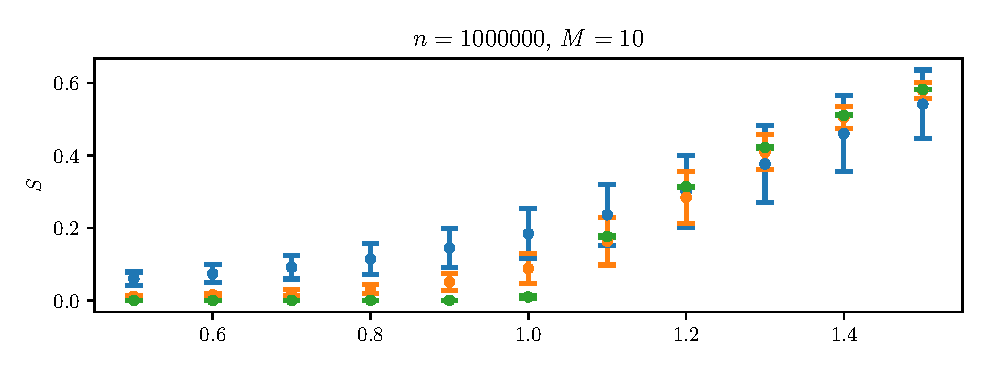
\includegraphics[scale=0.9]{GCC_ER.pdf}}\\
	\sidesubfloat[]{\includegraphics[scale=0.9]{GCC_geometric.pdf}}\\
	\sidesubfloat[]{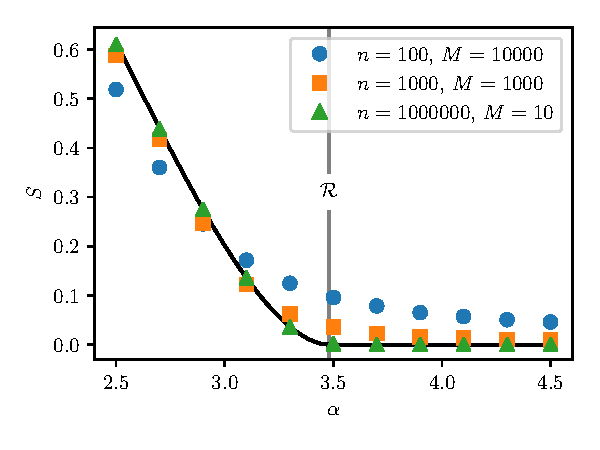
\includegraphics[scale=0.9]{GCC_Scalefree.pdf}}
	\caption{Numerical solution for $S$ of eq. \eqref{Single layer S final} and \eqref{Single layer u final} (solid black line), together with results on simulated networks. The critical point $\mathcal{R}$ computed using eq. \eqref{Boundary condition for single layer} is shown as a vertical gray line. Results of simulations are average over $M$ independently generated networks for various values of the number of nodes $n$ in the network. (A) Poisson degree distribution. (B) Geometric degree distribution. (C) Power law degree distribution.}
	\label{Figure: Single layer S simulation}
\end{figure}
}

\section{Generating connected networks}
\label{Section: Generating connected networks}

\subsection{Algorithm}

The knowledge of the degree distribution in the GCC can be used generate a connected component of a given degree distribution $r_k$ as it has been previously presented in \cite{bialas2008correlations}. To do so, we first determine a degree distribution $p_k$ fulfilling eq. \eqref{Degree distribution in GCC} for some target degree distribution $r_k$. Then we generate a network with degree distribution $p_k$ using the configuration model. Finally we take its GCC as our connected network. By construction the vertices in the GCC will have degree distribution $r_k$. Determining the factors $p_k$ is not immediate however since $u$ is an unknown which is itself a function of $p_k$. We propose an algorithm to determine it numerically.

First we isolate $p_k$ from eq. \eqref{Degree distribution in GCC} to get
\begin{align}
	p_k &= S \pi_k(u), \quad \text{with} \quad \pi_k(z) = \frac{r_k}{1 - z^k}
\end{align}
Inserting this in the expression \eqref{Single layer u final} for $u$, we get
\begin{align}
	u &= \frac{\sum_{k=1}^\infty k \pi_k(u) u^{k-1}}{\sum_{k=1}^\infty k \pi_k(u)}. \label{Fixpoint equation for u}
\end{align}
Therefore $u$ is a fixpoint of the function
\begin{align}
	\mu(z) = \frac{\sum_{k=1}^\infty k \pi_k(z) z^{k-1}}{\sum_{k=1}^\infty k \pi_k(z)}, \label{Defition of mu}
\end{align}
which is fully determined by the GCC degree distribution $r_k$. Note that for $r_1 = 0$, we have the fixpoint $u = 0$ and $p_k = r_k$ for all $k$. This is consistent with the fact that small component of a network produced with the configuration model have a probability $0$ to have loop \cite{newman2010networks}. Indeed if $p_1 = 0$ all components must have loops, therefore the probability to have small components is $0$ as well.

On the other hand $r_1 > 0$ implies $u > 0$. To approximate its value we define the sequence $u_{j+1} = \mu(u_j)$, with $u_0 = r_1$. This sequence will converge toward $u$ for large $j$. A proof of this statement is given in Appendix \ref{Appendix: Fixpoint convergence}.

In practice we can not deal evaluate infinite sums numerically, thus we need to choose a cutoff index $K$ for the sums such that
\begin{align}
	\sum_{k=K+1}^\infty k \pi_k(u) \ll 1.
\end{align}
For scale-free network with exponent smaller than 2 for example, this sum always diverges and thus this method is not applicable.

Once $u$ is approximated, we can compute the first $K$ probabilities $p_k$, which is sufficient to sample random numbers between $1$ and $K$ with relative probability $p_k$. If $K$ is chosen such that $r_k << 1$ for $k > K$, the degree distribution in the GCC closely approximate the distribution $r_k$.

\subsection{Erdos-Renyi reconstruction}

In order to test the algorithm presented, we choose the target connected degree distribution $r_k$ to be the degree distribution of the GCC of an Erdos-Renyi network. It is then expected that the reconstructed $p_k$ closely approximate a Poisson degree distribution.

The probability $p_k$ to have degree $k$ in an Erdos-Renyi network is given in eq. \eqref{pk for Erdos-Renyi}. Using eq. \eqref{Single layer u final} and \eqref{Single layer S final} to find $u$ and $S$ yield everything we need to be able to determine the GCC degree distribution $r_k$ from eq. \eqref{Degree distribution in GCC}. We can therefore use the algorithm on these $r_k$.

When computing $S$ for the original Poisson distribution, we should however be cautious, as the reconstructed $p_0$ will always be $0$. The expected resulting degree distribution, correctly normalized, is therefore
\begin{align}
	p_k = \frac{c^k}{k!} \frac{1}{e^{c} - 1}.
\end{align}
The expected bias ratio $r_k/p_k$ is shown for various mean degree $c$ and a cutoff constant $K = 10000$ in fig. \ref{Figure: Erdos-Renyi reconstruction} together with the same value computed from the algorithm presented above. As it can be seen, the agreement is very good. During the computations it has been observed that the closer the mean degree is to the critical value $c = 1$, the slower the fixpoint iteration converges.

\begin{figure}
	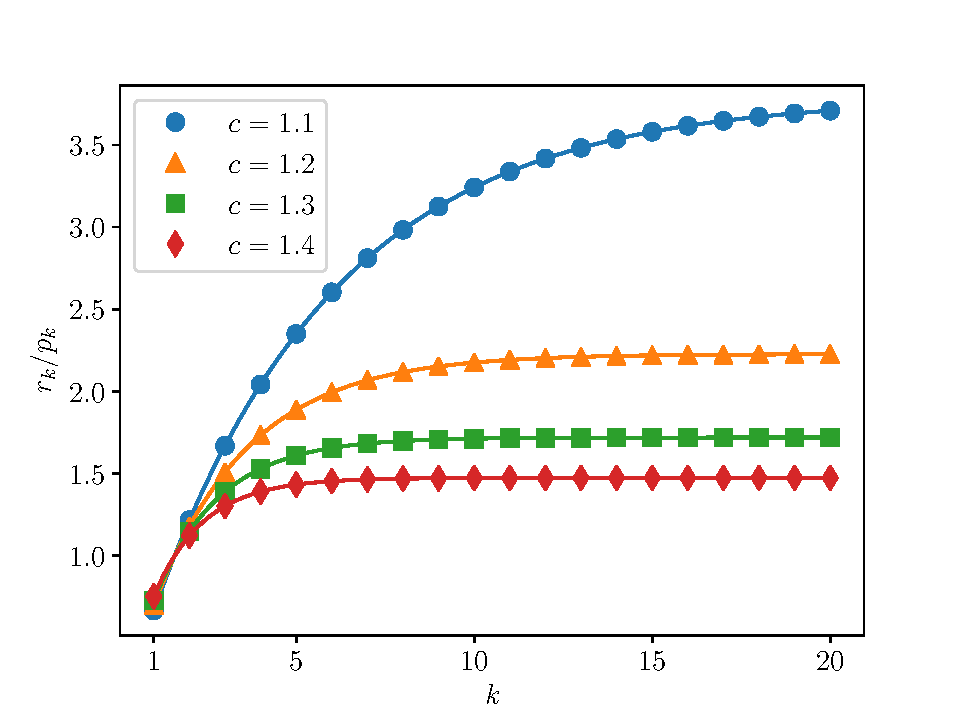
\includegraphics[width=0.8\textwidth]{ER_reconstruction.pdf}
	\caption{Bias factor $r_k/p_k$ for $r_k$ being the degree distribution of the GCC of an Erdos-Renyi network with various mean degree $c$ and cutoff constant $K = 10000$. The $p_k$ have been determined using the algorithm presented in the text. Solid line is the expected value $(1 - u^k)/S$ for the bias factor.}
	\label{Figure: Erdos-Renyi reconstruction}
\end{figure}

\subsection{Real world networks}

As an example of use of the algorithm presented, we apply it to real networks. We choose two by design connected network from the Konect network database \cite{kunegis2013konect}, the powergrid of the western states of the United States \cite{watts1998collective} and the road network of the state of California \cite{leskovec2008community} (the codes of the networks in the Konect database are respectively \code{UG} and \code{RO}). The power grid network is represented in fig. \ref{Figure: Network of western US powergrid}, while the Californian road network is not shown due to his high number of vertices ($n \approx 2 \times 10^6$).

The connected degree distribution $r_k$ is taken to be the empirical degree distribution of the real network considered. As a consequence, the cutoff constant $K$ is the maximal degree appearing in the network. Then, to sample the resulting degree distribution $p_k$, we simply take the number of vertex $d_k$ of degree $k$ to be the closest integer to $n p_k$, where $n$ is the total number of nodes. In the examples presented we use $n = 10^7$.

\begin{figure}
	\sidesubfloat[]{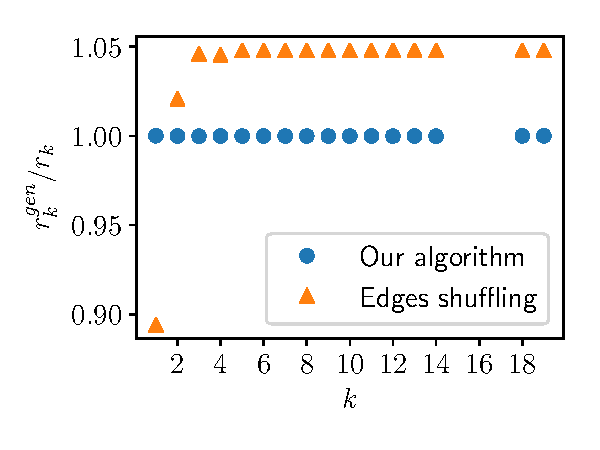
\includegraphics[width=0.45\textwidth]{real_US-power-grid.pdf}}\hfill
	\sidesubfloat[]{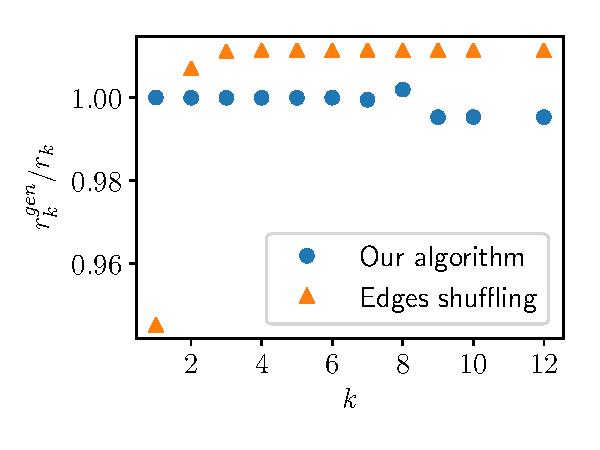
\includegraphics[width=0.45\textwidth]{real_roadNet-CA.pdf}}
	\caption{Plot of the ratio of the generated connected degree distribution $r^{gen}_k$ to the target degree distribution $r_k$ taken from a real network for our algorithm and the edges shuffling method. Missing values correspond to degree with probability $0$ to appear. (A) Western US power-grid network. (B) California road network.}
	\label{Figure: Real examples}
\end{figure}

We compare the degree distribution $r^{gen}_k$ of the GCC of the newly generated network with the target distribution $r_k$ by looking at the ratio $r^{gen}_k / r_k$. Resulting ratios are shown in fig. \ref{Figure: Real examples}, together with the results obtained by taking the GCC of the reshuffled network.

\todo[inline, color=yellow]{End of chapter 1 (for ref in todo list}


\chapter{Multiplex networks}
\label{Section: Multiplex networks}

\section{Introduction}

The concept of network can be extended by allowing different types of edges between the nodes of a network. Such generalized networks are called \newconcept{multiplex networks} or \newconcept{multi layers networks}. Among the real world example of such multiplex we find the various kind of connections between cities: transport connections (road, railroads, airlines), information connections (phone lines, internet connections) or supply connections (electricity, water).

However, such network can be more conveniently represented in a slightly different but equivalent way. We consider each type of edge to generate its own network. If we started with $L$ different type of edges, we therefore get $L$ networks, all sharing the same set of nodes. Conceptually it is similar to stack $L$ networks on top of each other, each network forming a \newconcept{layer} of the composed multi layers network (hence the name). An illustration of both representation of multiplex networks is shown in fig. \ref{Figure: Representations of multiplex networks} for a two layers network.

This representation also has the advantage of being readily generalizable to interdependent networks: rather than having nodes depend on exactly one node in each other layers, it may depends on nodes in other layer with some probability. This generalization allows to model any type of interdependent networks, which are ubiquitous in the real world, examples including interdepent infrastructure networks \cite{rinaldi2001identifying}, such as power-grids depending on their control network \cite{buldyrev2010catastrophic} and multiple networks of species interacting \cite{pocock2012robustness}. However, despite the strong modelling power of such interdependent networks, we restrict ourselves to the study of multiplex networks in this thesis.

\begin{figure}
	
\sidesubfloat[]{
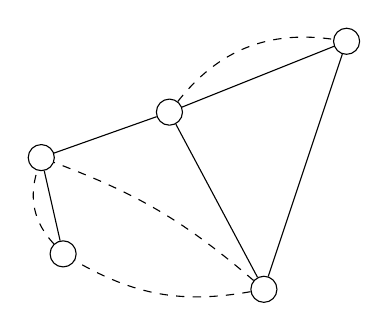
\begin{tikzpicture}[y=-1cm, scale=1.5]

	\node[node] (A) at (0.2, 0) {} ;
	\node[node] (B) at (1, 1.5) {} ;
	\node[node] (C) at (-0.7, 1.2) {} ;
	\node[node] (D) at (-0.5, -0,1) {} ;
	\node[node] (E) at (1.7, -0.6) {} ;

	\draw (A) -- (B) ;
	\draw (A) -- (D) ;
	\draw (A) -- (E) ;
	\draw (B) -- (E) ;
	\draw (C) -- (D) ;
	
	\draw[dashed] (A) to[bend left] (E) ;
	\draw[dashed] (B) to[bend left=20] (C) ;
	\draw[dashed] (B) to[bend right=10] (D) ;
	\draw[dashed] (C) to[bend left] (D) ;
\end{tikzpicture}
}\hspace{1cm}
\sidesubfloat[]{
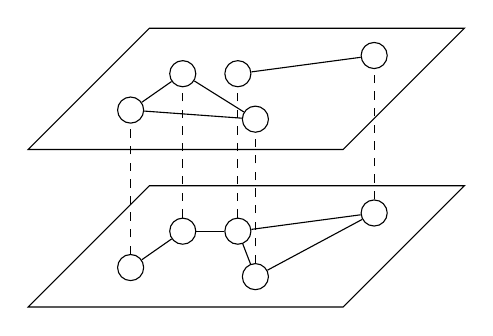
\begin{tikzpicture}[y = 2cm]
	\node[node] (A) at (0.2, 0, 0) {} ;
	\node[node] (B) at (1, 0, 1.5) {} ;
	\node[node] (C) at (-0.7, 0, 1.2) {} ;
	\node[node] (D) at (-0.5, 0, -0,1) {} ;
	\node[node] (E) at (1.7, 0, -0.6) {} ;
	
	\node[node] (A') at (0.2, 1, 0) {} ;
	\node[node] (B') at (1, 1, 1.5) {} ;
	\node[node] (C') at (-0.7, 1, 1.2) {} ;
	\node[node] (D') at (-0.5, 1, -0,1) {} ;
	\node[node] (E') at (1.7, 1, -0.6) {} ;
	
	\draw (-1.5, 0, -1.5) -- (2.5, 0, -1.5) -- (2.5, 0, 2.5) -- (-1.5, 0, 2.5) -- cycle ;
	\draw (-1.5, 1, -1.5) -- (2.5, 1, -1.5) -- (2.5, 1, 2.5) -- (-1.5, 1, 2.5) -- cycle ;
	
	\foreach \p in {A, B, C, D, E}
	{
		\draw[dashed] (\p) -- (\p') ;
	}
	
	\draw (A) -- (B) ;
	\draw (A) -- (D) ;
	\draw (A) -- (E) ;
	\draw (B) -- (E) ;
	\draw (C) -- (D) ;
	
	\draw (A') -- (E') ;
	\draw (B') -- (C') ;
	\draw (B') -- (D') ;
	\draw (C') -- (D') ;
	
	
\end{tikzpicture}
}
	\caption{Possible representations of a two layers network. (A) A network with two kinds of edges, straight solid lines and curved dashed ones. (B) Two networks in separate layers with corresponding nodes.}
	\label{Figure: Representations of multiplex networks}
\end{figure}

Thinking in term of layers also allows to reuse all quantities define in the context of single layer networks, such as the generating functions. We the extended quantity the same way as the original one, adding a subscript $i$ to its symbol to denote the fact that it applies to layer $i$, except if the symbol already has a subscript. In this case we add a superscript $(i)$.

Finally, we only consider that each layer of a multiplex network is independant to each other. This is most likely not true for real networks, but we restrict ourself to this case for simplicity.

\section{Giant viable cluster}
\label{Section: Giant Viable Cluster}

\subsection{Size of the GVC}
\label{Section: Size of GVC}

For single layer network, we are interested in the GCC as it is common for a system to be operational only if it is connected to the whole corresponding network. In the context of multiplex networks, the concept of connected component is extended by introducing \newconcept{viable clusters}. A viable cluster is defined as a subset of the multiplex network such that in every layer there is a path between any pair of vertices in that subset. Note that the path between two vertices must be totally included in the viable cluster, therefore the intersection of connected components is not in general a viable clusters as can be seen in fig. \ref{Figure: Intersection of connected is not viable}. This property is the rationale behind the definition of viable cluster as it is the minimal requirement to be sure that the resulting cluster are connected.

\begin{figure}
	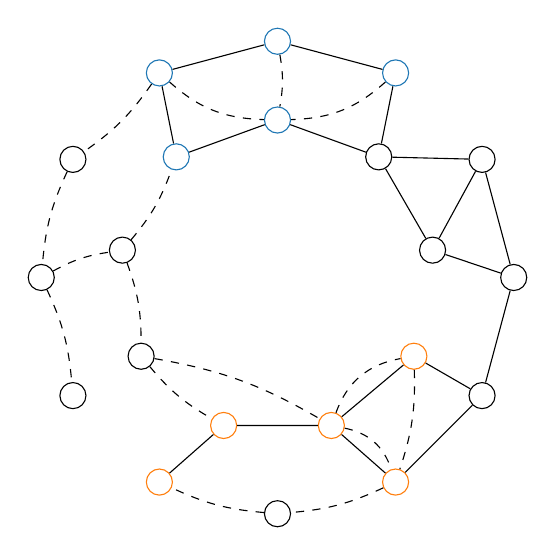
\begin{tikzpicture}
	\foreach \n in {1, 2, ..., 9}
	{
		\node (C\n') at ({2*sin(\n*360/9)}, {2*cos(\n*360/9)}) {} ;
	}
	
	
	\foreach \n in {1, 2, ..., 12}
	{
		\node (D\n') at ({3*sin(\n*360/12)}, {3*cos(\n*360/12)}) {} ;
	}
	
	\foreach \p in {D11, D12, D1, C8, C9}
	{
		\node[node, color=C0] (\p) at (\p') {} ;
	}
	
	\foreach \p in {C3, C4, C5, D5, D7}
	{
		\node[node, color=C1] (\p) at (\p') {} ;
	}
	
	\foreach \p in {C1, C2, C6, C7, D2, D3, D4, D6, D8, D9, D10}
	{
		\node[node] (\p) at (\p') {} ;
	}
	
	\draw (D7) -- (C5) -- (C4) -- (C3) -- (D4) -- (D5) -- (C4) ;
	\draw (D4) -- (D3) -- (D2) -- (C2) -- (D3) ;
	\draw (C2) -- (C1) -- (D2) ;
	\draw (C1) -- (D1) -- (D12) -- (D11) -- (C8) -- (C9) -- (C1) ;
	
	\draw[dashed] (D1) to[bend left=20] (C9) ;
	\draw[dashed] (D12) to[bend left=10] (C9) ;
	\draw[dashed] (D11) to[bend right=20] (C9) ;
	\draw[dashed] (D11) to[bend left=10] (D10) ;
	\draw[dashed] (D10) to[bend right=10] (D9) ;
	\draw[dashed] (D9) to[bend left=10] (D8) ;
	\draw[dashed] (D9) to[bend left=10] (C7) ;
	\draw[dashed] (C7) to[bend right=10] (C8) ;
	\draw[dashed] (C7) to[bend left=10] (C6) ;
	\draw[dashed] (C6) to[bend left=10] (C4) ;
	\draw[dashed] (C4) to[bend left] (C3) ;
	\draw[dashed] (C4) to[bend left] (D5) ;
	\draw[dashed] (C3) to[bend left=10] (D5) ;
	\draw[dashed] (D5) to[bend left=10] (D6) ;
	\draw[dashed] (D6) to[bend left=10] (D7) ;
	\draw[dashed] (C6) to[bend right=10] (C5) ;
\end{tikzpicture}
	\caption{Intersection of connected components of two layers of a multiplex networks. Edges in each layer are represented respectively with solid straight lines and curved dashed lines. The intersection is composed of the colored nodes, however there is no path in the intersection connecting the blue and orange nodes. Therefore the intersection results in two distinct viable clusters.}
	\label{Figure: Intersection of connected is not viable}
\end{figure}

Similar to the connected components in the single layer case, a viable cluster may occupy a non zero fraction of the network in the large $n$ limit. Such viable cluster is called the \newconcept{giant viable cluster} (GVC). Its existence and size are the main subjects of the discussion of this Chapter.

To be able to determine the size of the GVC, first let $g_0^{(i)}$ and $g_1^{(i)}$ be the generating functions of respectively the degree and the excess degree distribution in layer $i$. Moreover define $u_i$ as the probability that a vertex reached after following an edge in layer $i$ is not part of the giant viable cluster.

Then if we pick a vertex $v$ at random the probability $S$ that it is part a viable cluster $V$ can be written as
\begin{align}
	S &= P_0\left(\bigcap_{i = 1}^{L} \exists w \in N_i(v) \; w \in V \right),
\end{align}
that is vertex $v$ must have a neighbor in $V$ in each layer. By requiring that the layers are independent from one others, we can rewrite $S$ as a product
\begin{align}
	S &= \prod_{i = 1}^{L}  P_0^{(i)}\left(\exists w \in N_i(v) \; w \in V\right) \\
		&=\prod_{i = 1}^{L}  \left[1 - P_0^{(i)}\left(w \notin V \; \forall w \in N_i(v)\right) \right] \\
		&=\prod_{i = 1}^{L}  \left[1 - \sum_{k = 0}^{\infty} P_0^{(i)}\left(w \notin V \; \forall w \in N_i(v) | \deg{v} = k \right) p^{(i)}_k \right] \\
		&=\prod_{i = 1}^{L}  \left[1 - \sum_{k = 0}^{\infty} P_1^{(i)}\left(v \notin V | \deg{v} = k \right) p^{(i)}_k \right] \\
		&=\prod_{i = 1}^{L}  \left[1 - \sum_{k = 0}^{\infty} u_i^k p^{(i)}_k \right] \\
		&=\prod_{i = 1}^{L}  \left[1 - g_0^{(i)}(u_i) \right].\label{Multiplex GCC size final}
\end{align}
Here the reasoning is similar to the one leading to size of a connected component \eqref{Single layer S final} in the single layer case presented in Section \ref{Section: Giant connected component}. We can also find $u_j$ by a similar reasoning. First note that $1 - u_j$ is the probability that a vertex reached by following an edge in layer $j$ is in $V$. Which, due to the independence of the layers, can as before be written in the form
\begin{align}
	1 - u_j &= P_1^{(j)}\left(\bigcap_{i = 1}^{L} \exists w \in N_i(v) \; w \in V\right)\\
	&= \prod_{i = 1}^{L}  P_1^{(j)}\left(\exists w \in N_i(v) \; w \in V \right).
\end{align}
Moreover since the layers are independent, the fact that we reached $v$ by following an edge in layer $j$ to reach vertex $v$ is irrelevant in all other layers. However in layer $j$ this means that the degree distribution follows the distribution $q_k^{(j)}$ rather than $p_k^{(j)}$. Putting this together we get
\begin{align}
	1 - u_j &= \left[1 - \sum_{k = 0}^{\infty} u_j^k q_k^{(j)} \right] \prod_{\substack{i = 1 \\ i \neq j}}^{L}  \left[1 - \sum_{k = 0}^{\infty} u_i^k p^{(i)}_k \right] \\
	&= \left[1 - g_1^{(j)}(u_j) \right] \prod_{\substack{i = 1 \\ i \neq j}}^{L}  \left[1 - g_0^{(i)}(u_i) \right]. \label{Multiplex u final}
\end{align}
This equation has a trivial solution $u_j = 1$ for all layers, since by definition of the generating function \eqref{Definition of g0} we have
\begin{equation}
	g_0^{(j)}(1) = g_1^{(j)}(1) = 1.
\end{equation}
This also implies that the size of component $V$ is $0$. Hence to have a GVC it is necessary to find a non trivial solution to eq. \eqref{Multiplex u final}.

The size of the GVC as given by eq. \eqref{Multiplex GCC size final} and \eqref{Multiplex GCC size final} was first given in that form by Son \etal{} in \cite{son2012percolation}. In this paper Son \etal{} also treat a generalization in the form of the interdependent networks mentioned in the introduction of this chapter.

To rephrase this result in a mathematically more tractable way, we introduces some more notation. First consider that the degree distributions of the network's layers are determine by a finite parameter vector $\lambdavec = (\lambda_1, \lambda_2, \dots, \lambda_N)$, where $N$ is the number of parameters and does not need to equal the number of layers $N$. A typical parameter could be the mean degree of an Erdos Renyi graph for example.


Then, as in the single layer case, it is useful to express the $u_j$ as fixpoint of some function. In addition to providing a simple way of numerically solving eq. \eqref{Multiplex u final}, it can provide valuable information on the presence or absence of solutions as presented in Section \ref{Section: Interval arithemetic}.

To make the fixpoint nature of the $u_j$ manifest, we define the functions
\begin{align}
	\psi_j(\lambdavec, \zvec) = 1 - \left[1 - g_1^{(j)}(z_j) \right] \prod_{\substack{i = 1 \\ i \neq j}}^{L}  \left[1 - g_0^{(i)}(z_i) \right], \label{Definition of psi functions}
\end{align}
where $\zvec$ is the $L$ dimensional vector
\begin{align}
	\zvec = (z_1, z_2, \dots, z_L).
\end{align}
While we do not write it explicitly to avoid overcharging the notation, it is understood that the generating functions $g_0^{(i)}$ depend on the parameter vector $\lambdavec$.

Introducing a $L$ dimensional vector $\uvec$ and a $L$ dimensional function $\psi$ as respectively
\begin{align}
	\uvec &= (u_1, u_2, \dots, u_L) \\
	\psi(\zvec) &= (\psi_1(\zvec), \psi_2(\zvec), \dots, \psi_L(\zvec)),
\end{align}
we can compactly rewrite eq. \eqref{Multiplex u final} as
\begin{align}
	\uvec = \psi(\lambdavec, \uvec), \label{uvec as a fixpoint of psi}
\end{align}
which explicitly show that $\uvec$ is a fixpoint of the function $\psi$.

Finally, with this notation, the trivial solution to eq. \eqref{Multiplex u final} is written as
\begin{align}
	\uvec_T = (1, 1, \dots, 1). \label{Definition of multiplex trivial solution}
\end{align}
We have now gathered nearly as much informations about the GVC than we have about the GCC from the study we do of it in Section \ref{Section: Giant connected component}. However, while we have determined that the number of solutions to eq. \eqref{uvec as a fixpoint of psi} indicates if the networks is in a low or high connectivity phase, finding the boundary between the two is not as straightforward as it was in the single layer case. We return to that question in details in Section \ref{Section: Boundary condition for multilayer}, after we discuss one parameter multiplex networks, that allows easier visualization, and an algorithm to find the GVC.

\subsection{Single parameter multiplex networks}
\label{Section: Single parameter networks}

Graphical representation of solutions of multi dimensional equations such as eq. \eqref{Multiplex u final} is challenging. To avoid this problem we introduce single parameter networks. We define them as multiplex networks in which each layer has the same degree distribution. By letting the degree distribution depend on only one parameter $\lambda$, the dimension of the problem reduces to one, as in the single layer case, while still providing important inside in the difference brought by allowing multiple layers.

Mathematically, imposing constant degree distribution across layers implies that the generating functions are constant as well,
\begin{align}
	g^{(i)}_0(z) &= g_0(z), \\
	g^{(i)}_1(z) &= g_1(z), \qquad \forall i = 1, \dots, L.
\end{align}
Moreover by definition $u_j$ is the probability that, in the large $n$ limit, the probability that a vertex reached by following an edge is not part of the GVC. Having the same degree distribution in each layer, thus implies that the $u = u_j$ is the same for each layer.

Plugging these two observations into eq. \eqref{Multiplex u final} yields the single one dimensional equation for $u$
\begin{align}
	u &= 1 - \left[1 - g_1(u_j) \right] \prod_{\substack{i = 1 \\ i \neq j}}^{L}  \left[1 - g_0(u_i) \right] \\
		&= 1 - \left[1 - g_1(u) \right] \left[1 - g_0(u) \right]^{L - 1}. \label{Single parameter u final}
\end{align}
Similarly using eq. \eqref{Multiplex GCC size final} we find for $S$,
\begin{align}
	S = \left[1 - g_0(u) \right]^L. \label{Single parameter u final}
\end{align}

\begin{figure}
	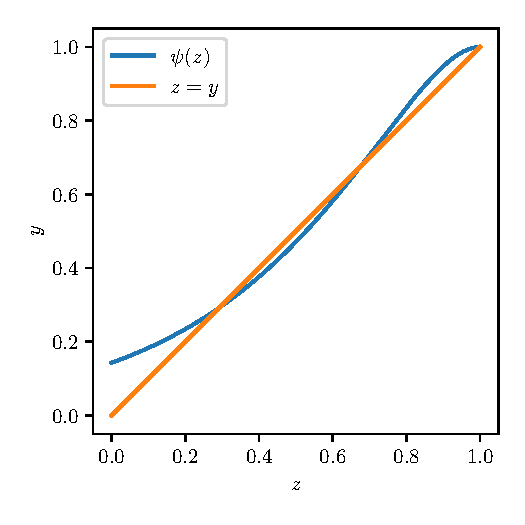
\includegraphics[scale=1]{single_param_u_solution_graphically.pdf}
	\caption{Graphical representation of eq. \eqref{Single layer u final} for multiplex network of two layers, both of which are Erdos Renyi graph with mean degree $c = 2.6$.}
	\label{Figure: Solution of u = psi(u) graphically for single param}
\end{figure}

Figure \ref{Figure: Solution of u = psi(u) graphically for single param} shows a graphical representation of eq. \eqref{Single parameter u final} for a two layer single parameter Erdos Renyi network. The main difference from the one layer case is that $\psi(z)$ has an inflexion point, as opposed to $g_1(z)$ in eq. \eqref{Single layer u final} that never does. As a consequence, eq. \eqref{Single parameter u final} can have more than two solutions and the condition \eqref{Boundary condition for single layer} does not hold. Indeed, while a new solution still appears when $\psi(z)$ is tangent to the identity line, this tangency point no longer appears at $z = 1$. This also indicates that the phase transition may be discontinuous for multiplex networks, a fact that we numerically verify for several examples in Section \ref{Section: Discontinuous phase transition}.

\subsection{Algorithm to find the viable clusters}

Similar to what we do in the single layer case, we would like to simulate and manipulate large networks. Therefore, algorithms must be carefully designed to be able to complete in a reasonable amount of time. The algorithm to find the GVC is significantly more complicated that the one presented in Section \ref{Section: Algorithm to find the GCC} because the paths we must consider to determine the GVC are dependent on the GVC itself: a path is valid if it is fully enclosed in the GVC, but a vertex is part of the GVC only if a path exist to all other vertices in the GVC. 

The main algorithm, adapted from \cite{baxter2012avalanche}, goes as follow:

\begin{enumerate}
	\item Add all nodes the set $\algoset{unprocessed}$ of unprocessed nodes.
	\item Create a new viable connected component guess $\algoset{guess}$ as an independent copy of $\algoset{unprocessed}$.
	\item Remove a node from $\algoset{unprocessed}$ and name it $v$.
	\item For each layer, exclude from $\algoset{guess}$ all nodes that are not part of the same connected component as $v$ in the subgraph spanned by the current $\algoset{guess}$.
	\item If the previous step modified $\algoset{guess}$ go back to it, else add $\algoset{guess}$ to the list of viable components and remove all nodes in it from $\algoset{unprocessed}$.
	\item If $\algoset{unprocessed}$ is empty terminate, else go to $2$.
\end{enumerate}

When the algorithm terminate, it has found all viable components of the multiplex network. To find the connected component in step 4 we use the procedure presented in Section \ref{Section: Algorithm to find the GCC}.

However, in this state, the algorithm may be crippling slow. To understand why observe that the most expensive viable component to determine tend to the smallest. Indeed for small components, step 4 may have to be repeated a large number of times until it has excluded most of the other vertices in the network. Moreover to be close to the critical point, where all layers are highly connected but no GVC emerges, is an aggravating factor. Not only the high connectedness of the layers makes step 4 longer to compute, but also the GCC intersection may be large and only composed of very small components that must individually be found among a large GCC intersection. For example for a two-layer multiplex network with each layer being an Erdos-Renyi network with $c = 2.3$ and $n = 10000$, we found that in average (over 10 runs) the intersection of the GCC occupied $74.3(6) \%$ of the network, but  no GVC exists and every of the viable component is composed of exactly one node. This makes the determination of the GVC prohibitively costly for large networks.\footnote{Baxter \etal{} do not mention the problem in the presentation of the algorithm on which we base our own \cite{baxter2012avalanche}, presumably because they do not present result of simulations in their paper.}

Since we are only interested in the size of the GVC, we can mitigate this problem by excluding all single layer connected components that are too small to be considered a GVC on their own. Only valid contender are the GCC of each layers, so we can immediately restrict our search to the intersections of the layers' GCC.

We then determine all connected components in the subgraph spanned by the vertices in the GCCs intersection. All components which occupy a fraction of the network smaller than a fixed level $\varepsilon$ are discarded. In this thesis we use $\varepsilon = 0.1\%$. The process is then repeated on the remaining vertices until no new vertices are excluded. Formally this preprocessing algorithm reads

\begin{enumerate}
	\item Compute the GCC in every layer of the network. Put each vertex that is in every GCC in $\algoset{initial}$.
	\item For every layer determine all connected components of the subgraph spanned by the vertices in $\algoset{initial}$.
	\item Remove from $\algoset{initial}$ all nodes that are part of a connected component occupying a fraction of the network smaller than $\varepsilon$ in any layer.
	\item If the previous step modified $\algoset{initial}$ go to 2, else terminate.
\end{enumerate}

The only change that must be done to the main algorithm is to modify step 1 such that only the vertices in $\algoset{initial}$ are added to $\algoset{unprocessed}$.

\section{Critical region}
\label{Section: Boundary condition for multilayer}

As mentioned at the end of Section \ref{Section: Size of GVC}, we would like to be able to determine under which conditions a multiplex network is in his high connectivity phase. To do this we want to find the critical region $\mathcal{R}$ in the parameter space between the low and high connectivity phase.

Before we can proceed to determining the critical region, we need to introduce some new concepts. First we define the residual functions
\begin{align}
	f_j(\lambdavec, \zvec) &= 1 - z_j - \left[1 - g_1^{(j)}(z_j) \right] \prod_{\substack{i = 1 \\ i \neq j}}^{L}  \left[1 - g_0^{(i)}(z_i) \right] \label{Definition fj} \\
		&= \psi_j(\lambdavec, \zvec) - z_j.
\end{align}
The functions $\psi_j(\lambdavec, \zvec)$ are the ones introduced in eq. \eqref{Definition of psi functions}. To get a compact representation of our problem, we gather all functions $f_j$ in the high dimensional function
\begin{align}
	f : \; &\mathbb{R}^N \times \unitinterval^L \rightarrow \mathbb{R}^L\\
	&(\lambdavec, \zvec) \mapsto F(\lambdavec, \zvec) = (f_1(\lambdavec, \zvec), f_2(\lambdavec, \zvec), \dots, f_L(\lambdavec, \zvec)) \label{Definition F} \\
		&\hphantom{(\lambdavec, \zvec) \mapsto F(\lambdavec, \zvec)} = \psi(\lambdavec, \zvec) - \zvec,
\end{align}
where $\unitinterval = [0, 1]$.

Then, since the functions $g_0^{(i)}$ and $g_1^{(i)}$ are analytic with respect to the $z_i$, the function
\begin{align}
	f_{\lambdavec} : \unitinterval^L &\rightarrow \mathbb{R}^L\\
		\zvec &\mapsto f(\lambdavec, \zvec),
\end{align}
is continuously differentiable for all parameter vectors $\lambdavec$. Therefore we can define Jacobi matrix $J_{\lambdavec}(\zvec)$ of $F_{\lambdavec}$ as having coefficients
\begin{align}
	\left[ J_{\lambdavec}(\zvec) \right]_{ij} = \frac{\partial f_i(\lambdavec,\zvec)}{\partial z_j} = \frac{\partial \psi_i(\lambdavec,\zvec)}{\partial z_j} - \delta_{ij}.
\end{align}

Now that we have introduced the quantities we will need, we can go back to the matter of solving eq. \eqref{Multiplex u final}. In term of the function $F$, this is equivalent for a given $\lambdavec$ to finding $\uvec \in \unitinterval^L$ that is a zero of $F$, i.e.
\begin{align}
	f(\lambdavec, \uvec) = 0. \label{Implicit equation}
\end{align}
Since this equation can be solve for all $\lambdavec$, it is tempting to try to express the $\uvec$ solving it has a function of $\lambdavec$, say $h(\lambdavec)$. However, eq. \eqref{Multiplex u final} is too complicated to be invertible, so we only know $h(\lambdavec)$ through the implicit equation
\begin{align}
	f(\lambdavec, h(\lambdavec)) = 0, \quad \forall \lambdavec \in U. \label{Implicit solution for F}
\end{align}
Now assume that $f$ (and not only $f_{\lambdavec}$) is continuously differentiable and that we are interested in $h(\lambdavec)$ such that it takes the value $\uvec^*$ for some $\lambdavec^*$, $h(\lambdavec^*) = \uvec^*$. The second condition is necessary to determine $h$ uniquely since eq. \eqref{Multiplex u final} may have multiple solutions, as shown in fig. \ref{Figure: Solution of u = psi(u) graphically for single param}.

If these conditions are fulfilled, the implicit function theorem tell us that in small neighbourhood $U$ around $\lambdavec^*$ we can find an uniquely defined continuous function $h(\lambdavec)$ that solve eq. \eqref{Implicit solution for F} if the Jacobi matrix $J_{\lambdavec^*}(\uvec^*)$ is not singular, that is if its determinant is not zero.

The result in which we are interested here comes from the contrapositive of this statement, namely that if for all neighbourhoods $U$ of $\lambdavec^*$ we can not find a uniquely defined continuous function $h$, then the determinant of the Jacobi matrix $J_{\lambdavec}(\uvec)$ must be zero, namely
\begin{align}
	\det\left[ J_{\lambdavec^*}(\uvec^*) \right] = 0 \label{Boundary condition},
\end{align}

We now prove that such situations arise if $\lambdavec^*$ is a critical point $\lambdavec^c$ of the phase transition between the absence and existence of a GVC, and therefore that eq. \eqref{Boundary condition} is a sufficient condition to find the critical region of such phase transition. This condition has previously been stated, without proof in \cite{baxter2012avalanche}. 

First consider a continuous phase transition. As shown in fig. \ref{Figure: Scheme of continuous and discontinuous phase transitions}, on one side of the phase transition occurring at $\lambdavec^c$ one solution exists, while on the other at least two do. Since the phase transition is continuous, for any $U$ open containing $\lambdavec^c$ we can define two distinct functions on $U$ that fulfil eq. \eqref{Implicit solution for F}, the trivial $h_T(\lambdavec) = \uvec_T$ and another function $h$ corresponding to the non trivial solutions, with $h(\lambdavec^c) = h_T(\lambdavec^c) = \uvec_T$. So the function $h$ of the implicit function theorem is not uniquely defined, regardless of the neighborhood $U$ chosen, and thus $\det\left[ J_{\lambdavec}(\uvec_T) \right] = 0$.

\begin{figure}
	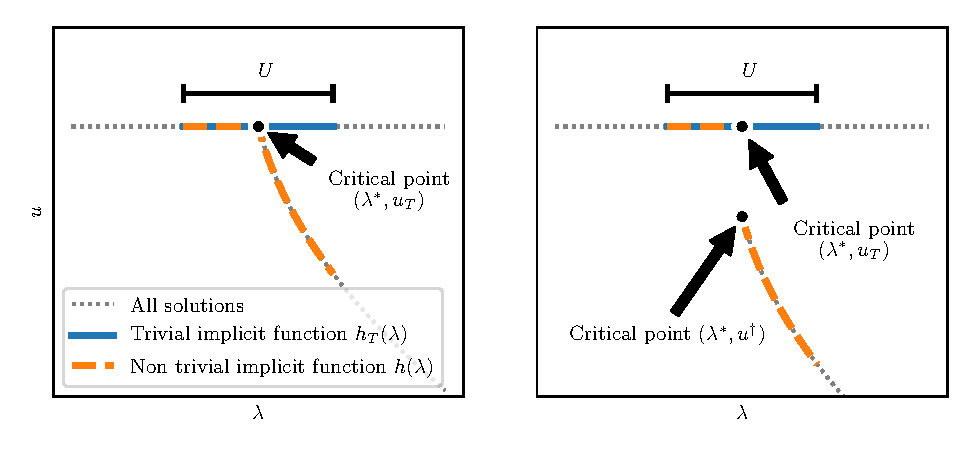
\includegraphics[width=\textwidth]{critical_point.pdf}
	\caption{Left panel: Scheme of a continuous phase transition. Right panel: Scheme of a discontinuous phase transition.}
	\label{Figure: Scheme of continuous and discontinuous phase transitions}
\end{figure}

On the other hand, let consider a discontinuous phase transition at $\lambdavec^c$. For any neighbourhood $U$ of $\lambdavec^c$ there are two sequences $(\lambdavec_n, \uvec_n)$ and $(\etavec_m, \vvec_m)$ with $\lambdavec_n, \etavec_m \in U$ for all $m, n \in \mathbb{N}$ such that
\begin{align}
	\lim_{n \rightarrow \infty} (\lambdavec_n, \uvec_n) &= (\lambdavec^c, \uvec^\dagger) \quad \text{ with } \uvec^\dagger \neq \uvec_T \\
	\lim_{m \rightarrow \infty} (\etavec_m, \vvec_m) &= (\lambdavec^c, \uvec_T) \\
	f(\lambdavec_n, \uvec_n) &= 0 \quad \forall n \\
	f(\etavec_m, \vvec_m) &= 0 \quad \forall m.
\end{align}
If we assume that an unique continuous function $h$ solving eq. \eqref{Implicit solution for F} exists, we would have
\begin{align}
	h(\lambdavec_n) &= \uvec_n \quad \forall n \\
	h(\etavec_m) &= \vvec_m \quad \forall m.
\end{align}
The continuity of $h$ would furthermore imply
\begin{align}
	h(\lambdavec^c) = \lim_{n \rightarrow \infty} h(\lambdavec_n) = \lim_{n \rightarrow \infty} \uvec_n = \uvec^\dagger,
\end{align}
but also
\begin{align}
	h(\lambdavec^c) &= \lim_{m \rightarrow \infty} h(\etavec_m) = \lim_{m \rightarrow \infty} \vvec_m = \uvec_T.
\end{align}
Since $\uvec_T \neq \uvec^\dagger$ as shown inf fig. \ref{Figure: Scheme of continuous and discontinuous phase transitions}, this gives raise to the contradiction $h(\lambdavec^c) \neq h(\lambdavec^c)$. Therefore our assumption must be false and no continuous function $h$ can be defined to solve eq. \eqref{Implicit solution for F}. So finally, we have $\det\left[ J(\lambdavec^c, \uvec) \right] = 0$, $\uvec$ being either $\uvec_T$ or $\uvec^\dagger$.

This conclude the proof, as it demonstrate that fulfilling eq. \eqref{Boundary condition} is always a necessary condition for the existence of a phase transition, regardless of the fact that it is or not continuous. Let stress here that in eq. \eqref{Boundary condition}, the $\lambdavec^*$ and $\uvec^*$ must also solve eq. \eqref{uvec as a fixpoint of psi}. Therefore to find the critical region $\mathcal{R}$, we must find a all couple $(\uvec, \lambdavec)$ that solve the system
\begin{align}
	\left\{ \begin{array}{l} \uvec = \psi(\lambdavec, \uvec) \\ \det\left[ J_{\lambdavec}(\uvec) \right] = 0. \end{array} \right. \label{Boundary condition full system}
\end{align}
Note that in the sequel we assume that in the high connectivity phase a GVC actually exists, but the theory presented in this chapter does not prove it, and to our knowledge no proof of this fact has been published.

Before going further, we briefly discuss the single layer case $L = 1$ in this framework. In that case the Jacobi matrix $J$ reduces to the scalar quantity
\begin{align}
	J_{\lambdavec}(u) = \frac{\partial}{\partial z} \left(g_1(z) - z\right)\rvert_{z = u} = g'_1(u) - 1.
\end{align}
Therefore the condition for the boundary $\det \left[ J_{\lambdavec}(u)\right] = 0$ becomes
\begin{align}
	g'_1(u) = 1.
\end{align}
As expected this condition is the same as the one given in eq. \eqref{Boundary condition for single layer} when discussing single layer networks.

\section{Interval arithmetic}
\label{Section: Interval arithemetic}

\subsection{Motivation}

In order to verify that eq. \eqref{Boundary condition} indeed gives the critical region $\mathcal{R}$ for a multiplex network, we need to introduce an independent numerical method to approximate it. This comes down to find the number of solutions of eq. \eqref{Multiplex u final} in the whole parameter space and then draw the boundary of the regions with a constant number of solution. However this leads to two problems.

First, standard algorithms to find zeros of functions are not guaranteed to find all zeros of a function. These algorithms usually find one solution at a time, the one being found depending on the initial guess solution provided by the user, no global information about the solution space being computed during the process. This causes immediate problem for our purpose, since missing a solution of eq. \eqref{Multiplex u final} may change our estimation of the boundary region by leading to the conclusion that some regions of the parameter space are part of trivial domain while they are not.

Secondly, the standard algorithms can only deal with one point of the parameter space at a time. This forces us to restrict our search on a discrete set of parameters. If this set is ill chosen, we may miss important features of the critical region. This second point is rather minor compared to the first. We indeed expect the critical region to be smooth and therefore restricting our analysis on any lattice should reasonably approximate it. We still mention this caveat however, since it can be solved using the same framework needed to solve the first issue.

Moreover, in Section \ref{Section: Single layer networks} we observed that for multiplex networks the phase transition displayed by eq. \eqref{Multiplex u final} seems to be discontinuous. However, to prove this fact we need to find some region between the trivial and non trivial solutions that can be proved to be exempt of any solution. As outlined above, standard zero finding algorithm are not suitable for such purpose.\footnote{While we put a special emphasis on proving that the phase transition we observe is discontinuous, the method we use is, to our knowledge, uncommon in the field of network science. More common method include using graphical solution of the kind presented in Fig. \ref{Figure: Solution of u = psi(u) graphically for single param} \cite{son2012percolation} or analytical arguments \cite{baxter2012avalanche}.}

To solve all these problems, we therefore introduce the field of \newconcept{interval arithmetic} and methods thereof that allows to rigorously guarantee presence or absence of solutions of equations in whole region of space.

\subsection{Theoretical foundation}
\label{Section: Theoretical foundation of IA}

First of all an \newconcept{interval} $Z$ is defined a set of the form
\begin{align}
	Z = \interval{a, b} = \set{x \in \mathbb{R} | a \leq x \leq b}.
\end{align}
The set of all intervals is denoted as $\mathbb{IR}$. The $N$-dimensional equivalent of an interval is an \newconcept{interval box} $\Zbox$, defined as the Cartesian product of $N$ intervals,
\begin{align}
	\Zbox = Z_1 \times Z_2 \times \cdots \times Z_N, \quad Z_k \in \mathbb{IR} \quad \forall k = 1, \dots, L
\end{align}
The set of all $N$-dimensional interval boxes is denoted $\mathbb{IR}^N$.

Given a function $\phi : \mathbb{R}^L \rightarrow \mathbb{R}^L$ we define a new interval valued function $\Phi$ such that
\begin{align}
	\Phi : \mathbb{IR}^L \rightarrow \mathbb{IR}^L \qquad \text{and} \qquad \zvec \in \Zbox \quad \Rightarrow \quad \phi(\zvec) \in \Phi(\Zbox). \label{Definition interval extension}
\end{align}
A function $\Phi$ with this property is called an \newconcept{interval extension} of $\phi$. In other words $\Phi(\Zbox)$ is guaranteed to contains the image of $\Zbox$ under $\phi$. Note that an interval extension is not unique, and we often would like to use the \emph{tightest} possible extension, meaning that we want $\Phi(\Zbox)$ to approximate $\phi(\Zbox)$ (i.e. the image of the set $\Zbox$ by $\phi$) as closely as possible. A perfect estimation is however not possible in general since the image of an interval box is not always itself an interval box.

Note that as oppose to $\phi$, its interval extension $\Phi$ is exactly representable numerically. This can be done by requiring the that the implementation of $\Phi$ includes numerical inaccuracy in such a way that the eq. \eqref{Definition interval extension} holds for the finite precision numerical result $\Phi(\Zbox)$. Hopefully good implementations, that respect this condition and are reasonably tight, can be found in existing libraries. In this thesis we use the implementation provided by the Julia packages \code{IntervalArithmetic.jl} \cite{intervalarithmetic} and \code{IntervalRootFinding.jl} \cite{intervalrootfinding}.

The properties of the interval extension allows to solve equations in a guaranteed way. To see that first consider an equation expressed as the fixpoint problem
\begin{align}
	\phi(\zvec) = \zvec,  \label{Interval arithmetic generic fixpoint}
\end{align}
and $\Phi$ an interval extension of $\phi$. There are many ways of defining $\phi$ to make an arbitrary equation equivalent to a fixpoint problem. For interval arithmetic the most common are Newton and Krawczyck  operators \cite{moore2009introduction, tucker2011validated}. As we use it below in Section \ref{Section: Discontinuous phase transition}, we introduce the latter in Appendix \ref{Appendix: Krawczyk operator}. However we will also use the more natural fixpoint displayed by eq. \eqref{uvec as a fixpoint of psi}.

Now that we have expressed a problem in term of a fixpoint, let the interval box $\Zbox$ contain a solution $\zvec^*$ of eq. \eqref{Interval arithmetic generic fixpoint}. By the definition \ref{Definition interval extension} of an interval extension and the fact that $\zvec^*$ is a fixpoint of $\phi$, we have
\begin{align}
	\zvec^* = \phi(\zvec^*) \in \Phi(\Zbox)
\end{align}
Since $\zvec^* \in \Zbox$ we can even say
\begin{align}
	\zvec^* \in \Zbox \cap \Phi(\Zbox).  \label{Generic solution refinement}
\end{align}

Therefore in general the relation between $\Zbox$ and $\Phi(\Zbox)$ can give information about the presence of solution in $\Zbox$. First if $\Zbox \cap \Phi(\Zbox) = \emptyset$, there can not be any solution of eq. \eqref{Interval arithmetic generic fixpoint} in $\Zbox$.

On the other hand, if $X \subseteq \Phi(\Zbox)$, we can use the fact that both $\Zbox$ and $\Phi(\Zbox)$ are interval boxes and thus are compact convex subspaces of $\mathcal{R}^N$. Brouwer fixpoint theorem can be used, which states that under such conditions, $\Phi(\Zbox)$ must have a fixpoint. As a consequence, $\Zbox$ must contain at least one solution. It has also been proven that for Newton and Krawczyck operators if $\Zbox$ is a subset of the interior of $\Phi(\Zbox)$, then the solution in $\Zbox$ is unique \cite{moore2009introduction, tucker2011validated}. We do not discuss the uniqueness further in this thesis though, as it is a technical point not necessary for our purpose.

Moreover, in the case where $\Zbox$ is neither outside of or included in $\Phi(\Zbox)$, we can not conclude anything about the number of solutions of eq. \eqref{Interval arithmetic generic fixpoint} in $\Zbox$. However, in this case $\Zbox$ could be bisected in the hope to be able to get more conclusive result on finer interval box.

To conclude this section, consider an interval box $\Zbox_0$ and the sequence $\Zbox_k$ of interval boxes recursively defined as
\begin{align}
	\Zbox_{k+1} = \Zbox_k \cap \Phi(\Zbox_k), \quad \forall k \in \mathbb{N}. \label{Generic refinement iteration}
\end{align}
Equation \eqref{Generic solution refinement} tells that all zeros present in the initial interval box $\Zbox_0$ are also present in $\Zbox_k$ for all $k$. By definition $\Zbox_{k+1} \subseteq \Zbox_k$, so iterating in the sequence for large $k$ can only yield a closer enclosure of the solutions in $\Zbox_0$. In fact, if $\Zbox_0$ contains one isolated solution $\zvec^*$ in its interior and $\zvec^*$ is an attractive fixpoint of $\phi$, then $\Zbox_k$ converges to $\set{\zvec^*}$ for large $k$. For Newton and Krawczyk operator it can actually be proven that it converges under weak assumptions \cite{moore2009introduction, tucker2011validated}.

This allows us to present a generic branch and bound algorithm to determine in principal, all fixpoints of a function $\phi$ in a starting interval box $\Zbox_0$, given an interval extension $\Phi$ of $\phi$:
\begin{enumerate}
	\item Define the set $\algoset{working}$ and add $\Zbox_0$ to it.
	\item If $\algoset{working}$ is empty go to 8, otherwise remove an interval box from $\algoset{working}$ and name it $\Zbox$.
	\item If the diameter of $\Zbox$ is smaller than some tolerance $\delta$ add $\Zbox$ to the set $\algoset{unkown}$ of interval box for which the algorithm is inconclusive and go to 2.
	\item Compute the contracted interval box $\ibox{C} = \Phi(\Zbox)$.
	\item If $\ibox{C} \subset \Zbox$, add $\Zbox$ to the set $\algoset{exist}$ of region in which a solution exists\footnote{For Newton and Krawczyk operator, checking if $\ibox{C}$ is in the interior of $\Zbox$ proves that the solution is unique. When using Krawczyk operator latter, this step is modified in that sense.} and go to $2$.
	\item If $\ibox{C} \cap \Zbox = \emptyset$, discard $\Zbox$ and go to $2$.
	\item Bisect the interval box $\ibox{C} \cap \Zbox$ along its largest edge and add both halves to $\algoset{working}$\footnote{Some care should be taken here in the case where $\ibox{C}$ end up being undefined or unbounded (this may happen with Newton and Krawczyk operator if the Jacobian is zero in $\Zbox$). See the implementation in the source code of \cite{intervalrootfinding} for details.}. Go to 2.
	\item Use the refinement iteration \eqref{Generic refinement iteration} until convergence is achieve on all elements of $\algoset{exist}$.
\end{enumerate}

Such algorithm is present in the package \code{IntervalRootFinding.jl} \cite{intervalrootfinding} which implementation we use latter with the Krawczyk operator\footnote{From a technical point of view, it should be noted that the version we use is the master branch in its state of the 31th of October 2018, with the inclusion of the pull request {\#}97. Also, while reviewed by and based on the previous work of the community, both Krawczyk operator and the generic branch and bound algorithm were written by the author, and should thus meet the same scepticism as the rest of this thesis.}.

\todoi{conclusion}

\subsection{Parametrized interval extension}
\label{Section: Parametrized interval extension}

As mentioned in the motivation of this section, interval arithmetic does not only give guaranteed results, it also allows to work with regions of a parameter space. To see that, consider a function
\begin{align}
	\phi(\lambdavec, \zvec) : \mathbb{R}^N \times \mathbb{R}^L \rightarrow \mathbb{R}^L,
\end{align}
for which we search a fixpoint
\begin{align}
	\phi(\lambdavec, \zvec) = \zvec.
\end{align}
Such parametrized problem, parametrized in the sense $\lambdavec$ can be seen as the parameters of the problem, have been previously discuss in the literature in the context of interval arithmetic, see for example \cite{neumaier1988enclosure}.

To find fixpoint of $\phi$, let first introduce $\Phi(\Lambdabox, \Zbox)$ an interval extension of $\phi(\lambdavec, \zvec)$. By definition of the interval extension \eqref{Definition interval extension}, we have
\begin{align}
	\phi(\lambdavec, \zvec) \in \Phi(\Lambdabox, \Zbox), \qquad \forall \lambdavec \in \Lambdabox, \forall \zvec \in \Zbox.
\end{align}
The crucial observation here is that, as a consequence, $\Phi(\Lambdabox, \Zbox)$ is an interval extension of the function
\begin{align}
	\phi(\lambdavec, \cdot) : \mathbb{R}^L &\rightarrow \mathbb{R}^L \\
	\zvec &\mapsto \phi(\lambdavec, \zvec)
\end{align}
for every $\lambdavec \in \Lambdabox$. This means that all reasoning using interval extension presented in the previous chapter can be applied at once for all value of $\lambdavec$ in $\Lambdabox$.

In particular this may allow to prove that a function has no solution for any $\lambdavec$ in some region of the parameter space, or on the opposite that it has a unique solution for every $\lambdavec$ of this region.

Too much should not be expected when working with large $\Lambdabox$ region. Indeed, in this case the interval extension may be far too broad to be able to conclude anything, making it of little use. However, as already mentioned in the previous section, in such case it is possible to bisect $\Lambdabox$ until it is small enough to provide conclusive results.


\subsection{Algorithm to approximate the critical region}

We would like to approximate the critical region $\mathcal{R}$ by an union of interval boxes, in the sense that we want a set of interval boxes $\Lambdabox_k$ such that
\begin{align}
	\mathcal{R} \subseteq \bigcup_k \Lambdabox_k.
\end{align}	
Obviously, we would this union to be the tightest possible around $\mathcal{R}$. However, we can not directly find such an union, the best we can do is to exclude interval boxes where the critical region can not be, either because we disprove the existence of any non trivial solution to eq. \eqref{uvec as a fixpoint of psi} on the whole parameter interval, or because we prove the existence of a non trivial solution for any parameter in the parameter interval. Technically, there is a third possibility using the system \eqref{Boundary condition full system}, which tell us we can exclude regions where the determinant of the Jacobian $J_{\lambdavec}$ can not be zero. However this last method would only give a numerical solution to our previous result, here we would like an independent approximation of the critical region to verify that  our result is correct. \todo{Mention if used latter}

To verify these criteria, we apply the logic we presented in Sections \ref{Section: Theoretical foundation of IA} and \ref{Section: Parametrized interval extension} to the function $\psi$ defined by eq. \eqref{Definition of psi functions}. Since we are interested in its fixpoints (as displayed by eq. \eqref{uvec as a fixpoint of psi}), this is fully compliant with the theory presented. Let $\Psi(\Lambdabox, \Zbox)$ be an interval extension of $\psi(\lambdavec, \zvec)$. Given a parameter interval box $\Lambdabox$ we can determine an approximations of all possible fixpoints of $\psi(\lambdavec, \cdot)$ using the root finding algorithm presented at the end of Section \ref{Section: Theoretical foundation of IA}. We consider three possible outcomes of the algorithm
\begin{enumerate}
	\item The algorithm yields at least one interval box not containing the trivial solution $\uvec_T$ in which a solution is guaranteed. In this case a non trivial solution exists, and therefore $\Lambda$ is fully enclosed in the non high connectivity phase.
	\item All interval boxes $\Zbox$ returned by the algorithm satisfy $\underline{Z_k} > 1 - \varepsilon$ for all $k = 1, \dots, L$, where $\underline{Z_k}$ is the lower bound of the component $k$ of $\Zbox$ and $\varepsilon$ is a small number \todo{choose for the real case}. This is needed to identify region where only the trivial solution $\uvec_T$ exists, as the algorithm is not able in general to conclude on the uniqueness of solution on the boundary of the search region. In this case we thus conclude that $\Lambda$ is included in the trivial region.
	\item If none of the above is satisfied, we can not conclude and we bisect $\Lambda$ until we can either conclude or its diameter falls under a threshold $\delta$.\todo{choose value}
\end{enumerate}

\todoi{conclude and speak about results}

\begin{figure}
	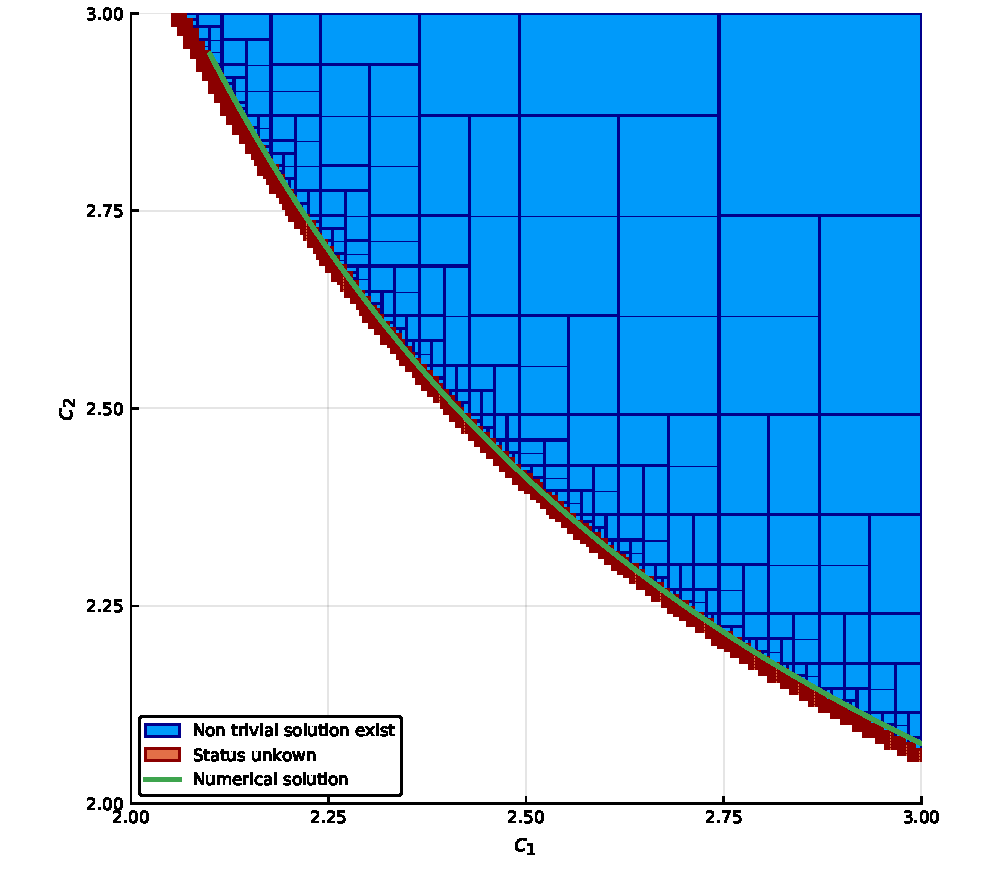
\includegraphics[width=0.8\textwidth]{two_layers_erdos_renyi_boundary.pdf}
	\caption{Phase diagram for a multiplex network composed of two Erdos-Renyi layer with mean degree $c_1$ and $c_2$. In the blue region a non trivial solution for $\uvec$ has been found, in the uncolored region only the trivial solution $\uvec_T$ exists and in the red region the algorithm was unable to conclude in favor of either case. The solid green line is the numerical solution to eq. \eqref{Multiplex u final} and \eqref{Boundary condition}.}
	\label{Figure: Regions and boundary}
	\todo[inline]{Make the plot more readable and less ugly}
	\todo[inline]{Find why the two methods seems drift away one from the other far from the center.}
\end{figure}

\subsection{Discontinuity of the phase transition}
\label{Section: Discontinuous phase transition}

A discontinuous phase transition implies a "gap" in between the trivial solution and the non trivial ones. Mathematically it is equivalent to the following
\begin{enumerate}
	\item There is a region $\mathcal{L}$ of the parameter space and a vector $\hat{\zvec} \in \mathcal{I}^L$, $\hat{\zvec} \neq \uvec_T$, such that for every parameter $\lambdavec \in \mathcal{L}$, all non trivial solutions $\uvec$ of eq. \eqref{Single parameter u final} have $\hat{z}_k > u_k$, for all $k = 1, \dots, L$.
	\item $\mathcal{L}$ covers the critical region $\mathcal{R}$, i.e. $\mathcal{R} \subseteq \mathcal{L}$.
\end{enumerate}

\begin{figure}
	\missingfigure{}
	\caption{Discontinuity check}
	\label{Figure: Discontinuity check}
\end{figure}

{\floatsetup[figure]{style=plain,subcapbesideposition=center}
\begin{figure}
	\sidesubfloat[]{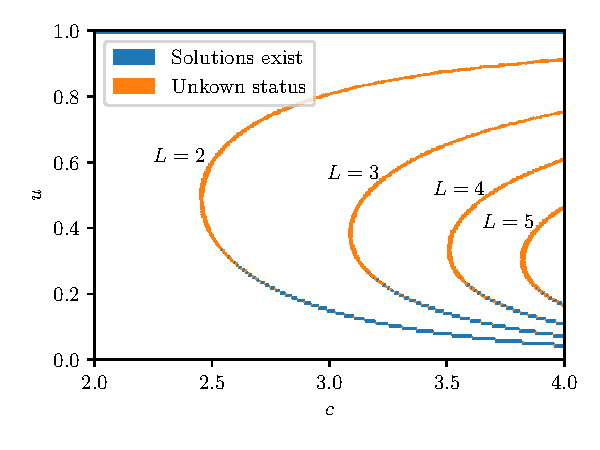
\includegraphics[scale=0.9]{multilayer_single_param_ErdosRenyiGraph.pdf}}\\
	\sidesubfloat[]{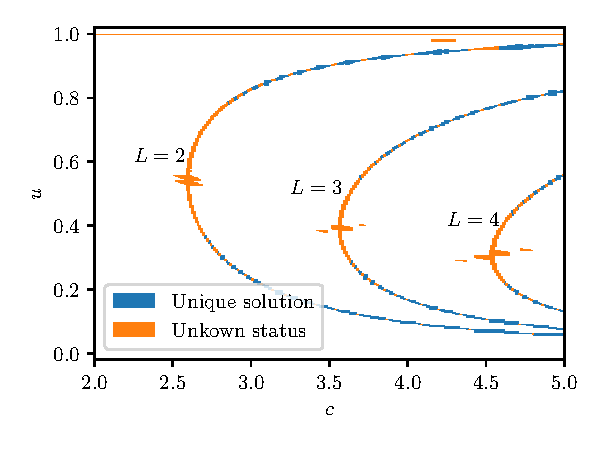
\includegraphics[scale=0.9]{multilayer_single_param_GeometricGraph.pdf}}\\
	\sidesubfloat[]{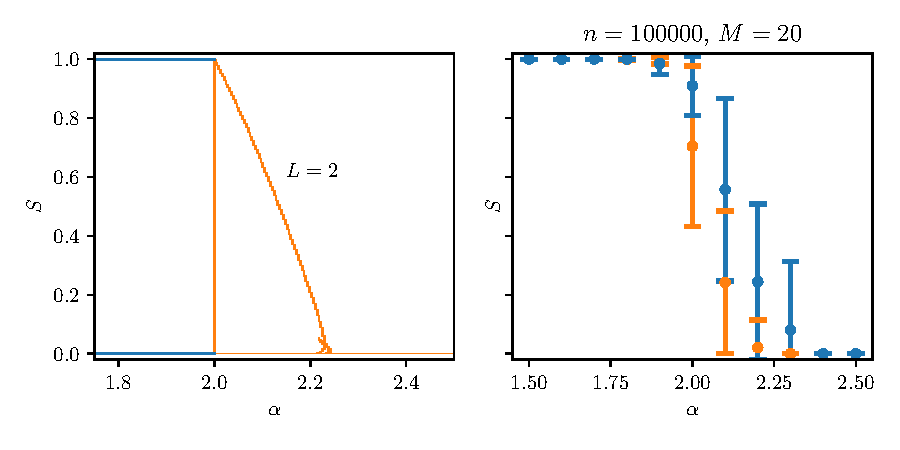
\includegraphics[scale=0.9]{multilayer_single_param_ScaleFreeGraph.pdf}}
	\caption{Solution of eq. \eqref{Single parameter u final} for various number of layers $L$. Exactly one solution exists for each $c$ in blue boxes, while uncolored part of the plot are guaranteed to contain no solutions. No conclusion can be made about existence of solution in the orange regions. These plots are sufficient to prove the discontinuity of the phase transition for Erdos-Renyi and exponential networks, but inconclusive for scale-free networks. (A) Erdos-Renyi network. (B) Exponential networks. (C) Scale-free networks.}
	\label{Figure: Multilayer single parameter}
	\todo[inline]{Reference figure somewhere}
	\todo[inline]{Speak about the solution z = 0 for SF alpha < 2}
	\todoi{Do something about alpha = 2}
\end{figure}
}

%--------------------------------------------
%	THESIS CONTENT - APPENDICES
%--------------------------------------------

\appendix  % Cue to tell LaTeX that the following "chapters" are Appendices

\chapter{Fixpoint iteration for connected networks generation}
\section{Convergence of the fixpoint iteration}
\label{Appendix: Fixpoint convergence}

First notice that the case $r_1 = 0$ is trivial, as described in the main text. We will therefore assume in this Appendix that $r_1 > 0$, immediately giving $\mu(0) = r_1 > 0$. Second, not that \eqref{Defition of mu} tells us that $z < 1$ implies $\mu(z) < 1$. From there we separate two cases:

If $u = 1$ is the unique solution of eq. \eqref{Fixpoint equation for u} then $\mu(z)$ must be continuous for $z \in [0, 1]$ and $\mu'(1) < 1$, making $u = 1$ and attractive fixpoint. On the other hand if there is another solution $u^*$ to eq. \eqref{Fixpoint equation for u}, it is the unique solution with $0 \leq u^* < 1$ since $\mu(z)$ is an increasing function of $z$, as it is demonstrated in Appendix \ref{Appendix: Monotonicity}. Moreover, since $\mu(0) > 0$ we have $\mu'(u^*) < 1$, which makes it an attracting fixpoint and makes $u = 1$ a repulsive one.

We can thus conclude that the fixpoint iteration proposed always converges and converges to the degenerate case $u = 1$ only if it is the unique possibility.

\section{Monotonicity of $\mu(z)$}
\label{Appendix: Monotonicity}

To prove that $\mu(z)$ is an increasing function, we compute its derivative with respect to $z$, which yields
\begin{align}
	\mu'(z) &= \left[\sum_{k = 1}^{\infty}k \pi_k(z)\right]^{-2} \left(s_1(z) + s_2(z)\right) \\
	s_1(z) &= \sum_{j, k}k j \pi_k'(z) \pi_j(z) \left( z^{k-1} -  z^{j-1}\right) \\
	s_2(z) &= \sum_{j, k} k (k - 1) j \pi_k(z) \pi_j(z) z^{k-2}.
\end{align}
The sum $s_1(z)$ can be rewritten as
\begin{align}
	s_1(z) &= \sum_{j > k} k j \left(\pi_k'(z) \pi_j(z) - \pi_j'(z) \pi_k(z)\right) \left(z^{k-1} -  z^{j-1}\right) \\
		&=\sum_{j > k} \frac{k r_k}{1 - z^k} \frac{j r_j}{1 - z^j} \frac{z^k - z^j}{z^2} \left(\frac{k}{z^{-k} - 1} - \frac{j}{z^{-j} - 1}\right)\\
		&=\sum_{j > k} k j \pi_k(z) \pi_j(z) \frac{z^k - z^j}{z^2} \left(\frac{k}{z^{-k} - 1} - \frac{j}{z^{-j} - 1}\right).
\end{align}
Using the fact that the function
\begin{align}
	f_z(\lambda) = \frac{\lambda}{z^{-\lambda} - 1}
\end{align}
is a decreasing function of $\lambda$ we can see that for $z \in [0, 1)$ and $j > k$ we have
\begin{align}
	z^k - z^j &\geq 0 \\
	\frac{k}{z^{-k} - 1} - \frac{j}{z^{-j} - 1} &\geq 0,
\end{align}
and thus $s_1(z) \geq 0$. Moreover each terms in $s_2(z)$ is non-negative, so we have $s_2(z) \geq 0$. We can therefore conclude that $\mu'(z) \geq 0$ and thus that $\mu(z)$ is an increasing function of $z$.

\chapter{Krawczyk operator}
\label{Appendix: Krawczyk operator}

\section{Mean value extension}

Before we can introduce Krawczyk operator and prove it has the properties we wish, we need to present a peculiar form of interval extension, the mean value extension. For this consider a differentiable function $a : \mathbb{R}^M \rightarrow \mathbb{R}$. Then by the mean value theorem, there is a vector $\xi$ lying on a straight path going from $\myvec{x}$ to $\myvec{y}$\footnote{Formally we can say that there is a real $t \in [0, 1]$ such that $\myvec{\xi} = (1 - t)\myvec{x} + t \myvec{y}$ fulfils eq. \eqref{Mean value theorem}},
\begin{align}
	a(\myvec{x}) - a(\myvec{y}) = \nabla a(\myvec{\xi}) \cdot (\myvec{x} - \myvec{y}). \label{Mean value theorem}
\end{align}
We note $A'(\ibox{X})$ and interval extension of $\nabla a(\myvec{x})$. Interval extension of function including derivatives can be computed either by explicitely knowing the derivatives or by automatic differentiation \cite{fike2012automatic}. The interval extension of the dot product $\cdot$ can be found by composing the interval extensions of the arithmetic operations\footnote{For all arithmetic operations, the optimal interval extension is known and actually implemented in \code{IntervalArithemetic.jl} \cite{intervalarithmetic}.}, which allows to define the interval valued function
\begin{align}
	A_{mv}(\ibox{X}) = a(m(\ibox{X})) + A'(\ibox{X}) \cdot (\ibox{X} - m(\ibox{X})), \label{Mean value extension}
\end{align}
with $m(\ibox{X})$ being the center of interval box $\ibox{X}$. Using the definition of interval extension \eqref{Definition interval extension} and the mean value theorem \eqref{Mean value theorem}, we see that
\begin{align}
	a(\myvec{x}) \in A_{mv}(\ibox{X}), \qquad \forall \myvec{x} \in \ibox{X},
\end{align}
and thus $A_{mv}(\ibox{X})$ is itself an interval extension of $a(\myvec{x})$, called the mean value extension of $a(\myvec{x})$. This proves useful in the next section, but is not in general the preferred way of extending a function as it requires computing its derivative.

\section{Fixpoint in Krawczyk operator}

Let consider a differentiable function $f : \mathbb{R}^M \rightarrow \mathbb{R}^M$ define over an interval box $\ibox{X}$ with interval extension $F$. We denote the Jacobian of $f$ as $f'$ and the interval extension of $f'$ as $F'$. Assume that $f'(m(\ibox{X})$ is not singular and hence invertible, which allows us to define $Y$ as its inverse. All these elements are needed to be able to define the Krawczyk operator of $f$
\begin{align}
	K(\ibox{X}) = m(\ibox{X}) - Y f(m(\ibox{X})) + \left[I - Y F'(\ibox{X})\right] (X - m(X)), \label{Krawczyk operator}
\end{align}
where $I$ is the identity matrix. Vector of intervals (interval boxes) and matrices of intervals follows the standard multiplication rules, where each component is an interval and arithmetic operations are replaced by on of their interval extension.

Krawczyk operator interest us because it fits in the framework presented in Section \ref{Section: Theoretical foundation of IA}: it is the interval extension of a function $k(\myvec{x})$ that has a fixpoint for solutions of the equation
\begin{align}
	f(\myvec{x}) = 0. \label{Krawczyk general equation to zero}
\end{align}
To prove this, we first write $k(x)$ explicitly as
\begin{align}
	k(\myvec{x}) = \myvec{x} - Y f(\myvec{x}).
\end{align}
Since $Y$ is not singular, $k(\myvec{x}^*) = \myvec{x}^*$ if and only if $f(\myvec{x}^*) = 0$. Moreover, for $k_i(\myvec{x})$ the $i$-th component $k(\myvec{x})$, $\left[f'(\myvec{x})\right]_i$ the $i$-th column of $f'(\myvec{x})$ and $e_i = (0, \dots, 1, \dots, 0)$ where the one is the $i$-th component, we have
\begin{align}
	\nabla k_i(\myvec{x}) = e_i - Y \left[f'(\myvec{x})\right]_i.
\end{align}
Applying eq. \eqref{Mean value extension} and using $F_i(\ibox{X})$ and $\ibox{X}_i$ to denote the $i$-th component of respectively $F(\ibox{X})$ and $X$, we find the mean value extension $K_i(\ibox{X})$ of $k_i(\myvec{x})$,
\begin{align}
	K_i(\ibox{X}) = m(\ibox{X}_i) - Y f_i(m(\ibox{X})) - \left[e_i - Y \left[F'(\ibox{X})\right]_i\right] \cdot (\ibox{X} - m(\ibox{X})).
\end{align}
Putting every component together, we end up on precisely the Krawczyk operator as given in eq. \eqref{Krawczyk operator}, thus proving that it is an interval extension of $k(\myvec{x})$. Therefore, following the reasoning presented in Section \ref{Section: Theoretical foundation of IA}, we have that $K(\ibox{X}) \subseteq \ibox{X}$ implies the existence of a solution in $K(\ibox{X})$ and that $K(\ibox{X}) \cap \ibox{X} = \emptyset$ implies the absence of solution in $\ibox{X}$.

Interestingly, while the Krawczyk operator was first introduced by Krawczyk in 1969 in \cite{krawczyk1969newton}, he only proved in this paper that it refines an interval $\ibox{X}$ around a solution $x^*$ of eq. \eqref{Krawczyk general equation to zero}. This is only in 1977 in \cite{moore1977test} that Moore made the observation and proved that Krawczyk operator can be used to determine the existence or absence of solution in a interval.

Note that in principle any matrix could be used in place of $Y$ in the definition of the Krawczyk operator, as we do not use the fact it is the inverse Jacobian in our demonstration. Using an approximation of the inverse of $f'(\myvec{x}^*)$ is however useful as it ensure that the iteration \eqref{Generic refinement iteration} converges towards the solution and that it does so faster than linearly \cite{krawczyk1969newton}.

Finally, note that this dependence on the inverse of $f'(\myvec{x})$ is in general a liability. Indeed, if it is zero for a solution $\myvec{x}^*$, the algorithm described in Section \ref{Section: Theoretical foundation of IA} is not able to prove its existence. Indeed, if $X$ contains $\myvec{x}^*$ such that $f'(\myvec{x}^*) = 0$, then $Y x = \mathbb{IR}^M$ for any vector or interval box $\myvec{x}$. As a consequence we have $K(\ibox{X}) = \mathbb{IR}^M$, which is surely not included in $\ibox{X}$.

In this regard, Krawczyk method is however more reliable. Its alternative, the Newton method, indeed requires that the Jacobian $f'(\myvec{x})$ is regular everywhere in the interval box $\ibox{X}$ considered \cite{moore2009introduction, tucker2011validated}, while the Krawczyk only need in principle that it is the case for the solution.\footnote{In fact by using extended interval arithmetic, the problem can be avoided altogether with Newton method \cite{hansen1978globally}, but we decided not use this generalization here for simplicity.}

%--------------------------------------------
%	BIBLIOGRAPHY
%--------------------------------------------

\printbibliography[heading=bibintoc]{}

% \printindex{}

\end{document}